\documentclass[prt,twocolumn,floatfix,nofootinbib]{revtex4}
\usepackage{amssymb}
\usepackage{amsmath}
\usepackage{graphicx,color,dcolumn,booktabs,bm}
\usepackage{longtable,lscape}
\usepackage{txfonts}
\usepackage{overpic}
\usepackage{indentfirst}
\usepackage{cases}
\usepackage{multirow}
\usepackage{epstopdf}
\usepackage{ulem}
\usepackage[colorlinks,
            citecolor=blue,
            anchorcolor=red,
            menucolor=red,
            linkcolor=red,
            filecolor=red,
            runcolor=red,
            urlcolor=blue,
            frenchlinks=false]{hyperref}
%\newtheorem{theorem}{Theorem}
%\newtheorem{remark}[theorem]{Remark}
%\newtheorem{solution}[theorem]{Solution}
%\newtheorem{summary}[theorem]{Summary}
%\newenvironment{proof}[1][Proof]{\noindent\textbf{#1.} }{\ \rule{0.5em}{0.5em}}
%\usepackage{tikz}
\setcounter{MaxMatrixCols}{10}
\def\lrpartial{\buildrel\leftrightarrow\over\partial}
\allowdisplaybreaks

\linespread{1.1}
\begin{document}
%\title{Ground-state baryons and tetraquarks with one and two heavy quarks: Masses, magnetic moments}
\title{Masses and magnetic moments of hadrons with open heavy quarks up to two in MIT bag model: baryons and tetraquarks}

\author{Wen-Xuan Zhang$^{1}$}
\author{Hao Xu$^{1,2}$}
\author{Duojie Jia$^{1,2}$
\footnote{Corresponding author}}
\email{jiadj@nwnu.edu.cn}
\author{Xue-Qian Li$^{3}$}

\affiliation{ $^1$Institute of Theoretical Physics, College of Physics and
Electronic Engineering, Northwest Normal University, Lanzhou 730070, China \\
$^2$Lanzhou Center for Theoretical Physics, Lanzhou University, Lanzhou, 730000,China \\
$^3$School of Physics Science, Nankai University, Tianjin 300071, China \\ }


\begin{abstract}
In this work, we compute masses and magnetic moments of the heavy baryons and tetraquarks with one and two open heavy flavors in MIT bag model in an unified way. In addition to the parameters of MIT bag model and the charm and bottom quark masses extracted from the heavy mesons with $J^{P}=1^{-}$, we incorporate a term of extra binding energy into MIT bag model, which is supposed to exist among heavy quarks ($c$ and $b$) and between heavy and strange quarks in the literatures. Numerical calculations are made for all light mesons, open heavy hadrons with heavy flavors of at least two, predicting the mass of doubly charmed baryons to be $M(\Xi_{cc})=3.604$ GeV, $M(\Xi_{cc}^{\ast})=3.714$ GeV, and that of the strange isosinglet tetraquark $ud\bar{s}\bar{c}$ with $J^{P}=0^{+}$ to be $M\left(ud\bar{s}\bar{c}\right)=2.934$ GeV. We find that the state mixing due to chromomagnetic interaction is sizable as indicated by comparing with the perturbative computation.

{\normalsize PACS number(s):12.39Jh, 12.40.Yx, 12.40.Nn}
{\normalsize Key Words: Heavy baryons, heavy tetraquark, Mass, Magnetic moment}
\end{abstract}
\maketitle
\date{\today}


\maketitle\section{Introduction}
In 2017, the LHCb Collaboration at CERN discovered the doubly charmed baryon $\Xi_{cc}^{++}$ with $J^{P}={1/2}^{+}$ and the measured mass $3621.40\pm 0.78$ MeV \cite{Aaij:2017ueg}. The observation provides an important experimental information about the strength of interaction between two heavy quarks, and makes it possible to resolve the question whether the tetraquarks $QQ\bar{q}\bar{q}$ with two open heavy quarks $Q$ and two light antiquarks $\bar{q}$ are stable or unstable against decaying into two $Q\bar{q}$ mesons \cite{Karliner:2017qjm,Eichten:2017ffp,Luo:2017eub}.
More recently, LHCb Collaboration reported the first exotic state $X_{0}(2900)$ with open heavy flavors and mass $2866\pm 7$ MeV \cite{LHCb:2020kd}. in Ref.~\cite{Karliner:2020vsi}, this state has been interpreted as an isosinglet tetraquark $cs\bar{u}\bar{d}$ . These findings, among others, arrouse great interest in doubly heavy baryons and tetraquarks.

Up to date, various approaches, including potential quark models and bag model, have been employed to explore doubly heavy hadrons \cite{Fleck:1989mb,Ebert:2004ck,Bernotas:2012nz,He:2004px,Karliner:2014gca,Liu:2018euh} , and heavy tetraquarks\cite{}. See Refs \cite{Ali:2017jda,Liu:2019zoy} for recent reviews. As masses and other properties are of valuable in identifying and/or finding them experimentally, a systematic computation of mass and other properties remains to be done within an unified framework. For instance, a mass prediction about $3620$ MeV \cite{Ebert:2004ck,Karliner:2014gca} for the doubly charmed baryon $\Xi_{cc}$, larger about $100$ MeV than that measured in 2002 by the SELEX Collaboration at Fermilab \cite{Moinester:2002uw}(awaiting confirmation), helps to identify the LHCb-reported $\Xi_{cc}^{++}$ as the first doubly charmed baryon \cite{Aaij:2017ueg} eventually.

In this work, we employ MIT bag model to systematically study masses and magnetic moments of open heavy baryons and tetraquarks with one and two heavy flavors.
By the way, masses and other properties of light mesons, heavy mesons in their ground-states are also calculated. For the baryon states of $\Xi_{c}$, $\Xi_{b}$, $\Xi_{bc}$, $\Omega_{bc}$ with $J^{P}={\frac{1}{2}}^{+}$ with chromomagnetic mixing, we compute their mass splittings due to CMI and the respective properties via numerical variational method, compared to perturbative treatment of chromomagnetic interactions. We find that the MIT bag model, with extra binding energy term supposed to exist among heavy quarks ($c$ and $b$) and strange quarks in the literatures, can reconcile heavy hadrons with light hadron in their masses and other properties. Our mass calculation reproduces the measured masses of heavy hadrons below the accuracy of $40$ MeV, from which we proceed to predict the masses and other properties of the tetraquarks with one and two open heavy quarks.

It is well known that bag model \cite{DeGrand:1975cf} embodies two primary features of quantum chromodynamics (QCD): asymptotic freedom at short distance and confinement at long distance. The simple structure of the model enables us to describe mesons($q\bar{q}$), baryons($qqq$) and even hadrons made of multiquarks. In the past few decades, bag model have been applied to describe the doubly heavy baryons\cite{Fleck:1989mb,He:2004px, Bernotas:2012nz} and multiquark hadrons, including light exotic baryons with five and seven nonstrange quarks \cite{Strottman:1979qu}. A large running strong coupling $\alpha_{s}$ was applied in Ref. \cite{He:2004px} to evaluate the masses of doubly heavy baryons, and in Refs.~\cite{Haxton:1980mc,Aerts:1980rf} a Coulomb-like interaction is derived between heavy quarks in a bag.

This paper will be organized as follows. In Sec.~\ref{Method}, we review some basic relations of MIT bag model, including chromomagnetic interaction (CMI) among the quarks in bag.
In Sec.~\ref{Parameters}, a systematic numerical calculation is performed for the established light and heavy baryons, with the optimal set of parameters obtained and the results for masses and other properties reproduced.
In Sec.~\ref{Hadrons}, we present a detailed predictions for masses and other propeties for doubly heavy baryons and the tetraquarks with open heavy quarks up to two. The paper ends with summary and conclusions in Sec.~\ref{Discussions}.


\section{Method for MIT bag model with CMI}\label{Method}
\subsection{Mass Formula}
Treating hadron as a sphere bag, MIT bag model provides an approach to estimate masses and other properties of hadrons in their ground states \cite{Johnson:1975zp,DeGrand:1975cf},
in which the chromomagnetic interaction is derived from the energy of a sphere-like gluon field interacting with quark fields in bag \cite{DeGrand:1975cf}.
The mass formula of hadron in MIT bag model is,
\begin{equation}\label{MBm}
    M\left(R\right)=\sum_{i=n,s,c,b} n_{i}\omega_{i}+\frac{4}{3}\pi R^{3}B-\frac{Z_{0}}{R}+\langle \Delta H \rangle,
\end{equation}
\begin{equation}\label{freq}
    \omega_{i}=\left(m_{i}^{2}+\frac{x_{i}^{2}}{R^2}\right)^{1/2},
\end{equation}
where the first term is the kinematic energy of all quarks in bag with radius $R$, the second is the volume energy of bag with bag constant $B$, the third is the zero-point-energy (ZPE) with coefficient $Z_{0}$, and $\langle \Delta H \rangle$ is interaction energy among quarks in bag, on which we will address in this work.
Here in Eq. (\ref{MBm}), $n_{i}$ is number of quark or antiquark in bag with mass $m_{i}$ and flavor $i$, where $i$ can be the light nonstrange quarks $n=u,d$, the strange quark $s$, the charm quark $c$ and the bottom quark $b$. The value of $R$ is to be determined variationally, and the dimensionless parameters $x_{i}=x_{i}(mR)$ are related to the bag radius $R$ by an transcendental eigen-equation
\begin{equation}\label{transc}
    \tan x_{i}=\frac{x_{i}}{1-m_{i}R-\left(m_{i}^{2}R^{2}+x_{i}^{2}\right)^{1/2}}.
\end{equation}

The interaction energy $\langle \Delta H \rangle=B_{EB}+ M_{CMI}$ is composed of two energy terms:

(1) The binding energy $B_{EB}$, due mainly to the short-range chromoelectric interaction between quarks (and/or antiquarks), which is spin-independent.
Owing to its smallness for the relativistic light quarks $n$($=u, d$), this energy, scales mainly as $-\sum \alpha_{s}/r_{ij}$, becomes sizable when both of two quarks $i$ and $j$ are massive and moving nonrelativistically.
In present work, we treat this energy as sum of the pair binding energies $B_{QQ^{\prime}}$ ($B_{Qs}$) between heavy quarks and between heavy quark $Q$ and strange quark $s$ \cite{Karliner:2014gca,Karliner:2017elp,Karliner:2018bms}.
The net effect for this chromoelectric interaction amounts to introduction of five binding energies $B_{cs}$, $B_{cc}$, $B_{bs}$, $B_{bb}$ and $B_{bc}$,
which are extractable from heavy mesons for the quark pair configuration $\boldsymbol{\bar{3}}_{c}$ and can be scaled to other color configurations.

(2) The chromomagnetic interaction energy, due to perturbative gluon exchange between quarks (antiquarks) $i$ and $j$,
\begin{equation}\label{CMI}
    M_{CMI}=-\sum_{i<j} \left(\boldsymbol{\lambda_{i}}\cdot \boldsymbol{\lambda_{j}}\right) \left(\boldsymbol{\sigma_{i}}\cdot \boldsymbol{\sigma_{j}}\right)C_{ij},
\end{equation}
with $\boldsymbol{\lambda}_{i}$ the Gell-Mann matrices, $\boldsymbol{\sigma}_{i}$ the Pauli matrices, and $C_{ij}$ the CMI parameter. In MIT bag model, the parameters $C_{ij}$ are given by
\begin{equation}\label{Cij}
    C_{ij}=3\frac{\alpha_{s}\left(R\right)}{R^{3}}\bar{\mu}_{i}\bar{\mu}_{j}I_{ij},
\end{equation}
\begin{equation}\label{muBari}
   \bar{\mu}_{i}=\frac{R}{6} \frac{4\alpha_{i}+2\lambda_{i}-3}{2\alpha_{i}\left(\alpha_{i}-1\right)+\lambda_{i}},
\end{equation}
\begin{equation}\label{Iij}
    I_{ij}=1+2\int_{0}^{R} \frac{{\rm d}r}{r^{4}} \bar{\mu}_{i}\bar{\mu}_{j}=1+F(x_{i}, x_{j}),
\end{equation}
where $\alpha_{i}\equiv\omega_{i}R$, $\lambda_{i}\equiv m_{i}R$, $\alpha_{s}\left(R\right)$ is the running strong coupling, $\bar{\mu}_{i}$ is the reduced magnetic moment without electric charge,
and $I_{ij}$ and $F(x_{i}, x_{j})$ are a rational function of $x_{i}$ and $x_{j}$, given explicitly by\cite{DeGrand:1975cf}.
\begin{equation}\label{F}
    \begin{aligned}
        F(x_{i}, x_{j})={\left(x_{i} {\rm sin}^{2}x_{i}-\frac{3}{2}y_{i}\right)}^{-1} {\left(x_{j} {\rm sin^{2}}x_{j}-\frac{3}{2}y_{j}\right)}^{-1} \\
        \left\{-\frac{3}{2}y_{i}y_{j}-2x_{i}x_{j} {\rm sin}^{2}x_{i} {\rm sin}^{2}x_{j} +\frac{1}{2}x_{i}x_{j}\left[2x_{i} {\rm Si}(2x_{i}) \right.\right.\\
        \left.\left. +2x_{j} {\rm Si}(2x_{j}) -(x_{x}+x_{j}) {\rm Si}(2(x_{x}+x_{j})) \right.\right.\\
        \left.\left. -(x_{x}-x_{j}) {\rm Si}(2(x_{x}-x_{j})) \right] \right\}
    \end{aligned}
\end{equation}
where $y_{i}=x_{i}-{\rm cos}(x_{i}){\rm sin}(x_{i})$, $x_{i}$ the root of Eq. (\ref{transc}) for a given $m_{i}R$, and
\begin{equation}
    {\rm Si}(x)=\int_0^x\ \frac{sin(t)}{t}dt.
\end{equation}

In some applications of bag model \cite{Haxton:1980mc,Aerts:1980rf,Carlson:1982er,He:2004px,Fleck:1989mb}, the parameter $\alpha_{s}$ takes, inspired by QCD renormalization, a semiempirical form
\begin{equation}\label{alphaS}
    \alpha_{s}(R)=\frac{2\pi n}{9} \frac{1}{ln\left[\gamma+{\left(R\Lambda_{QCD}\right)}^{-n}\right]},
\end{equation}
where exponent $n=1$ or 2, with 1 prefered for suppressing the value of $\alpha_{s}$, $\Lambda_{QCD}$ is the QCD scale ranging from $0.2$ GeV to $0.5$ GeV, and $\gamma$ is prefactor used to avoid divergence.
Similar to Ref.~\cite{He:2004px}, we take $\Lambda_{QCD}=0.281$ GeV to set
\begin{equation}\label{alphaS-mine}
    \alpha_{s}(R)=\frac{0.296}{{\rm ln}\left[1+{\left(0.281R\right)}^{-1}\right]},
\end{equation}
which is plotted in FIG.~\ref{fig:alphaS}. Among four lines showing the running of $\alpha_{s}$ in the plot, the solid line shows notable variation and corresponds to a relative lower value of $\alpha_{s}$.
In the case of light hadrons, the hadron masses evaluated by Eq.~(\ref{alphaS-mine}) are listed in Table \ref{tab:lighthadron}, compared to that predicted by original MIT bag model.

\begin{figure}[!ht]
    \begin{center}
        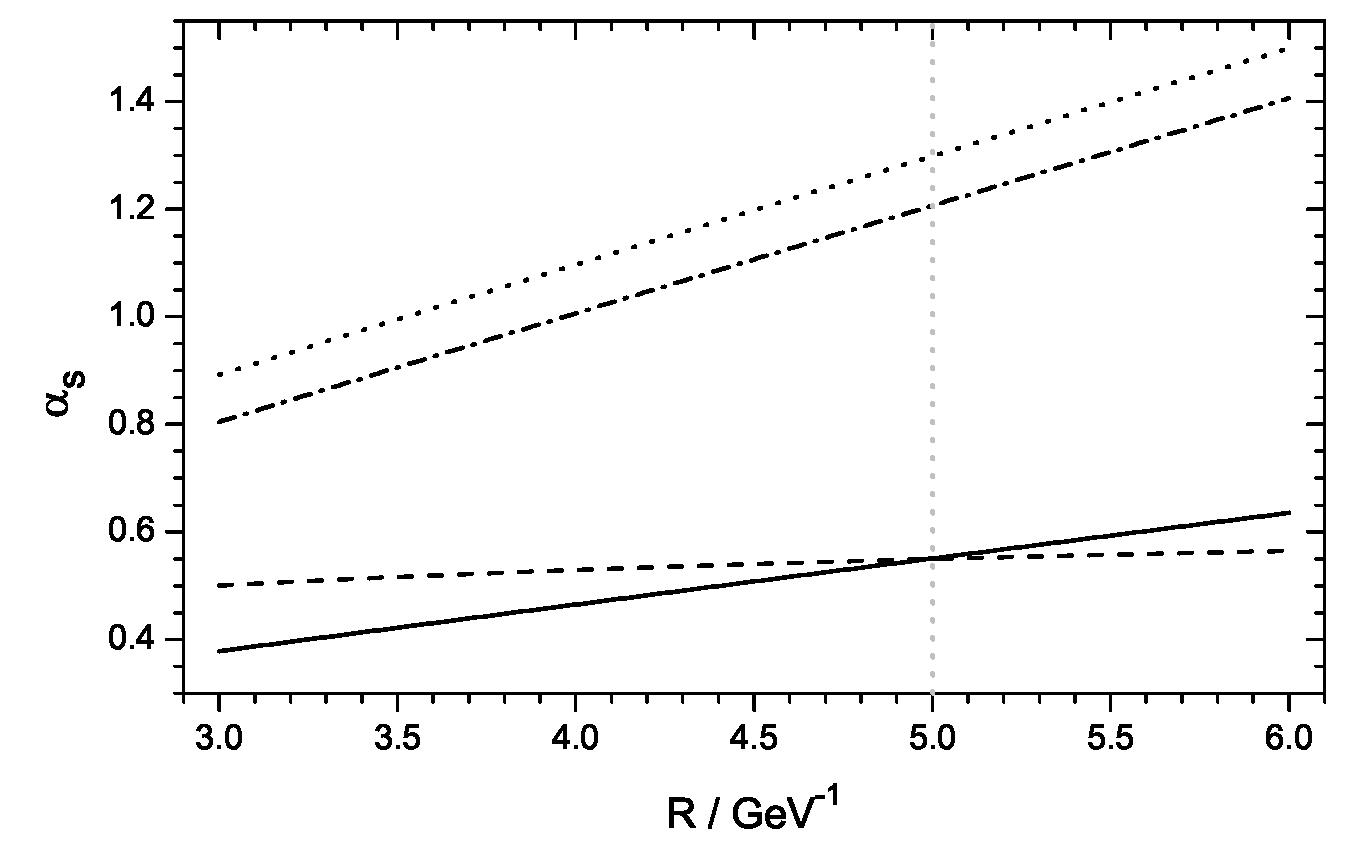
\includegraphics[width=0.47\textwidth]{AlphaS.eps}
    \end{center}
    \caption{Four running behaviors of strong coupling.
    Bag radius $R$ ranges from $3\,{\rm GeV}^{-1}$ to $6\,{\rm GeV}^{-1}$, and the standard radius is set to be $5\,{\rm GeV}^{-1}$ ($\approx 1\,{\rm fm}$) for checking.
    The solid line represents our result (\ref{alphaS-mine}) while the dashed line corresponds to Eq.~(\ref{alphaS}) with $\gamma=2.847$ and $\Lambda_{QCD}=0.281\,{\rm GeV}$. The dotted line shows Eq.~(\ref{alphaS}) with $\gamma=1$ and $\Lambda_{QCD}=0.281\,{\rm GeV}$. The dotdashed line indicates that of Ref.~\cite{He:2004px}.}
    \label{fig:alphaS}
\end{figure}

\renewcommand{\tabcolsep}{0.39cm}
\renewcommand{\arraystretch}{1.3}
\begin{table}[!htbp]
    \caption{Bag radius $R$ (in GeV$^{-1}$) and mass prediction $M_{bag}$ (in GeV) obtained from this work ($Z_{0}=1.83$) and original MIT bag model for light hadrons, compared to the measured mass $M_{exp}$ (in GeV) being isospin-averaged.}
    \label{tab:lighthadron}
    \begin{tabular}{cccccc}
        \hline\hline
        \multirow{2}{*}{State} & \multicolumn{2}{c}{MIT bag\cite{Johnson:1975zp}} & \multicolumn{2}{c}{\rm This\ work} & \multirow{2}{*}{$M_{exp}$} \\
        \cline{2-3} \cline{4-5}
        & $R$ & $M_{bag}$ & $R$ & $M_{bag}$ \\ \hline
        $N$               &5.00      &0.938      &5.22      &0.932      &0.939  \\
        $\Delta$          &5.48      &1.233      &5.33      &1.241      &1.232  \\
        $\Lambda$         &4.95      &1.105      &5.26      &1.096      &1.116  \\
        $\Sigma$          &4.95      &1.144      &5.22      &1.137      &1.193  \\
        $\Xi$             &4.91      &1.289      &5.27      &1.282      &1.318  \\
        $\Sigma^{\ast}$   &5.43      &1.382      &5.38      &1.383      &1.385  \\
        $\Xi^{\ast}$      &5.39      &1.529      &5.42      &1.529      &1.533  \\
        $\Omega$          &5.35      &1.672      &5.46      &1.677      &1.672  \\
        $\pi$             &3.34      &0.280      &4.31      &0.348      &0.137  \\
        $\omega$          &4.71      &0.783      &4.55      &0.776      &0.783  \\
        $K$               &3.26      &0.497      &4.34      &0.561      &0.496  \\
        $K^{\ast}$        &4.65      &0.928      &4.63      &0.918      &0.894  \\
        $\phi$            &4.61      &1.068      &4.70      &1.064      &1.019  \\
        \hline\hline
    \end{tabular}
\end{table}

Given the parameter values of the quark mass $m_{i}$, bag constant $B$, the ZPE coefficient $Z_{0}$ and strong coupling constant $\alpha_{s}(R)$ depending on bag radius $R$, one can apply variational method to determine the respective bag radius $R$ for each hadron and the respective $x_{i}$ through Eq. (\ref{transc}). Then, it is straightforward to use Eqs. (\ref{MBm}),(\ref{freq}) and (\ref{CMI}) to compute the ground-state masses and other static properties (magnetic moments, the charge radius) of the hadrons ranging from mesons to tetraquarks. Meanwhile, we also give a first-order perturbative computation for the CMI-mixed states by treating Eq. (\ref{CMI}) as a pertubation.

We stress that for a given hadronic state there is in principle a unique set of the solution $x_{i}$ and $R$ corresponding to respective bag dynamics, as indicated by our computation. Owing to $(x_{i},R)$-dependence of the $\langle \Delta H \rangle$, a simple and analytic mass formula is lacking for the hadrons with chromomagnetic-mixing since for that purpose one has to first diagonalize the CMI matrices before the variational analysis, which amounts to a higher-order algebraic equations.


\subsection{Chromomagnetic Structure}
To evaluate the mass splitting due to the chromomagnetic interaction in Eq.~(\ref{CMI}), in which $\boldsymbol{\lambda_{i}}$ should be replaced by $-\boldsymbol{\lambda_{i}^{\ast}}$ for a antiquark, one has to diagonalize
the CMI matrix for given hadron multiplets with certain $J^{P}$ quantum number to give the respective mass splitting \cite{Luo:2017eub} within the multiplets. For this, we list all the flavor-spin-color wavefunctions for mesons, baryons and tetraquark systems considered in this work, and present relevant formulas of the color and spin factors for them.

A ground-state meson with color wavefunction $\phi^{M}=\left| q_{1}\bar{q}_{2} \right\rangle$
can be one of two spin states (of vector and scalar like ):
\begin{equation}\label{spinM}
    \chi_{1}^{M}={\left| q_{1}\bar{q}_{2} \right\rangle}_{1}, \quad \chi_{2}^{M}={\left| q_{1}\bar{q}_{2} \right\rangle}_{0},
\end{equation}
where subscript $J=0,1$ outside the bracket denotes the total spin of hadron. The spin-color wavefunctions of mesons with spin $J=0,1$ are then
\begin{equation}\label{colorspinM}
    \phi^{M}\chi_{1}^{M}={\left| q_{1}\bar{q}_{2} \right\rangle}_{1}, \quad \phi^{M}\chi_{2}^{M}={\left| q_{1}\bar{q}_{2} \right\rangle}_{0}.
\end{equation}

A baryon with color wavefunctions $\phi^{B}=\left| {\left(q_{1}q_{2}\right)}^{\bar{3}} q_{3} \right\rangle$
can be in one of three spin states
\begin{equation}\label{spinB}
    \begin{aligned}
        \chi_{1}^{B}={\left| {\left(q_{1}q_{2}\right)}_{1} q_{3} \right\rangle}_{3/2}, \\
        \chi_{2}^{B}={\left| {\left(q_{1}q_{2}\right)}_{1} q_{3} \right\rangle}_{1/2}, \\
        \chi_{3}^{B}={\left| {\left(q_{1}q_{2}\right)}_{0} q_{3} \right\rangle}_{1/2},
    \end{aligned}
\end{equation}
where $\left(q_{1}q_{2}\right)$ stands for a diquark with spin $J=1$ or $0$ in color configuration $\boldsymbol{\bar{3}}_{c}$.

To find wavefunction for a hadron, the flavor symmetry has to be considered. For a flavor-symmetric wavefunction of $\left(q_{1}q_{2}\right)$, with isospin $I=1$ or identical flavors, we use a symbol $\delta_{12}^{S}=1$.
For a flavor-asymmetric wavefunction with $I=0$, a symbol $\delta_{12}^{A}=1$ will be used. For two quarks $q_{1}$ and $q_{2}$ with different flavors which goes beyond isospin symmetry, one can use $\delta_{12}^{S}=\delta_{12}^{A}=1$.
With the help of Pauli principle, one can write three flavor-spin-color wavefunctions for a baryon
\begin{equation}\label{colorspinB}
    \begin{aligned}
        \phi^{B}\chi_{1}^{B}={\left| {\left(q_{1}q_{2}\right)}_{1}^{\bar{3}} q_{3} \right\rangle}_{3/2} \delta_{12}^{S}, \\
        \phi^{B}\chi_{2}^{B}={\left| {\left(q_{1}q_{2}\right)}_{1}^{\bar{3}} q_{3} \right\rangle}_{1/2} \delta_{12}^{S}, \\
        \phi^{B}\chi_{3}^{B}={\left| {\left(q_{1}q_{2}\right)}_{0}^{\bar{3}} q_{3} \right\rangle}_{1/2} \delta_{12}^{A}.
    \end{aligned}
\end{equation}

A possible situation is that the states mix due to chromomagnetic interaction.
For example, for the doubly heavy baryons $\Xi_{bc}$ and $\Xi_{bc}^{\prime}$ with flavor structure $(bc)s$ the use of $\delta_{12}^{S}=\delta_{12}^{A}=1$ is not enough to distinguish the two configurations $\phi^{B}\chi_{2}^{B}$ and $\phi^{B}\chi_{3}^{B}$ solely in terms of their $J^{P}$ quantum numbers. Thus, the physical state must be one of the mixing states of them. See sect.~\ref{Parameters} for the details of colormagnetic mixing.

A tetraquark with color structure $\boldsymbol{6}\otimes\boldsymbol{\bar{6}}$ or $\boldsymbol{\bar{3}}\otimes\boldsymbol{3}$, with the respective color wavefunctions,
\begin{equation}\label{colorT}
    \phi_{1}^{T}=\left| {\left(q_{1}q_{2}\right)}^{6} {\left(\bar{q}_{3}\bar{q}_{4}\right)}^{\bar{6}} \right\rangle, \quad
    \phi_{2}^{T}=\left| {\left(q_{1}q_{2}\right)}^{\bar{3}} {\left(\bar{q}_{3}\bar{q}_{4}\right)}^{3} \right\rangle,
\end{equation}
can be one of the following six states
\begin{equation}\label{spinT}
    \begin{aligned}
        \chi_{1}^{T}={\left| {\left(q_{1}q_{2}\right)}_{1} {\left(\bar{q}_{3}\bar{q}_{4}\right)}_{1} \right\rangle}_{2}, \quad
        \chi_{2}^{T}={\left| {\left(q_{1}q_{2}\right)}_{1} {\left(\bar{q}_{3}\bar{q}_{4}\right)}_{1} \right\rangle}_{1}, \\
        \chi_{3}^{T}={\left| {\left(q_{1}q_{2}\right)}_{1} {\left(\bar{q}_{3}\bar{q}_{4}\right)}_{1} \right\rangle}_{0}, \quad
        \chi_{4}^{T}={\left| {\left(q_{1}q_{2}\right)}_{1} {\left(\bar{q}_{3}\bar{q}_{4}\right)}_{0} \right\rangle}_{1}, \\
        \chi_{5}^{T}={\left| {\left(q_{1}q_{2}\right)}_{0} {\left(\bar{q}_{3}\bar{q}_{4}\right)}_{1} \right\rangle}_{1}, \quad
        \chi_{6}^{T}={\left| {\left(q_{1}q_{2}\right)}_{0} {\left(\bar{q}_{3}\bar{q}_{4}\right)}_{0} \right\rangle}_{0},
    \end{aligned}
\end{equation}
which provide twelve base wavefunctions
\begin{equation}\label{colorspinT}
    \begin{aligned}
        \phi_{1}^{T}\chi_{1}^{T}={\left| {\left(q_{1}q_{2}\right)}_{1}^{6} {\left(\bar{q}_{3}\bar{q}_{4}\right)}_{1}^{\bar{6}} \right\rangle}_{2} \delta_{12}^{A}\delta_{34}^{A}, \\
        \phi_{2}^{T}\chi_{1}^{T}={\left| {\left(q_{1}q_{2}\right)}_{1}^{\bar{3}} {\left(\bar{q}_{3}\bar{q}_{4}\right)}_{1}^{3} \right\rangle}_{2} \delta_{12}^{S}\delta_{34}^{S}, \\
        \phi_{1}^{T}\chi_{2}^{T}={\left| {\left(q_{1}q_{2}\right)}_{1}^{6} {\left(\bar{q}_{3}\bar{q}_{4}\right)}_{1}^{\bar{6}} \right\rangle}_{1} \delta_{12}^{A}\delta_{34}^{A}, \\
        \phi_{2}^{T}\chi_{2}^{T}={\left| {\left(q_{1}q_{2}\right)}_{1}^{\bar{3}} {\left(\bar{q}_{3}\bar{q}_{4}\right)}_{1}^{3} \right\rangle}_{1} \delta_{12}^{S}\delta_{34}^{S}, \\
        \phi_{1}^{T}\chi_{3}^{T}={\left| {\left(q_{1}q_{2}\right)}_{1}^{6} {\left(\bar{q}_{3}\bar{q}_{4}\right)}_{1}^{\bar{6}} \right\rangle}_{0} \delta_{12}^{A}\delta_{34}^{A}, \\
        \phi_{2}^{T}\chi_{3}^{T}={\left| {\left(q_{1}q_{2}\right)}_{1}^{\bar{3}} {\left(\bar{q}_{3}\bar{q}_{4}\right)}_{1}^{3} \right\rangle}_{0} \delta_{12}^{S}\delta_{34}^{S}, \\
        \phi_{1}^{T}\chi_{4}^{T}={\left| {\left(q_{1}q_{2}\right)}_{1}^{6} {\left(\bar{q}_{3}\bar{q}_{4}\right)}_{0}^{\bar{6}} \right\rangle}_{1} \delta_{12}^{A}\delta_{34}^{S}, \\
        \phi_{2}^{T}\chi_{4}^{T}={\left| {\left(q_{1}q_{2}\right)}_{1}^{\bar{3}} {\left(\bar{q}_{3}\bar{q}_{4}\right)}_{0}^{3} \right\rangle}_{1} \delta_{12}^{S}\delta_{34}^{A}, \\
        \phi_{1}^{T}\chi_{5}^{T}={\left| {\left(q_{1}q_{2}\right)}_{0}^{6} {\left(\bar{q}_{3}\bar{q}_{4}\right)}_{1}^{\bar{6}} \right\rangle}_{1} \delta_{12}^{S}\delta_{34}^{A}, \\
        \phi_{2}^{T}\chi_{5}^{T}={\left| {\left(q_{1}q_{2}\right)}_{0}^{\bar{3}} {\left(\bar{q}_{3}\bar{q}_{4}\right)}_{1}^{3} \right\rangle}_{1} \delta_{12}^{A}\delta_{34}^{S}, \\
        \phi_{1}^{T}\chi_{6}^{T}={\left| {\left(q_{1}q_{2}\right)}_{0}^{6} {\left(\bar{q}_{3}\bar{q}_{4}\right)}_{0}^{\bar{6}} \right\rangle}_{0} \delta_{12}^{S}\delta_{34}^{S}, \\
        \phi_{2}^{T}\chi_{6}^{T}={\left| {\left(q_{1}q_{2}\right)}_{0}^{\bar{3}} {\left(\bar{q}_{3}\bar{q}_{4}\right)}_{0}^{3} \right\rangle}_{0} \delta_{12}^{A}\delta_{34}^{A}.
    \end{aligned}
\end{equation}

We list all relevant color wavefunctions in Appendix A and spin wavefunctions in Appendix B. With them, one can evaluate the color and spin factors in Eq.~(\ref{CMI}) with the help of the following formulas
\begin{equation}\label{colorfc}
    {\left\langle \boldsymbol{\lambda_{i}}\cdot \boldsymbol{\lambda_{j}} \right\rangle}_{nm}=
    \sum_{\alpha=1}^{8} Tr\left(c_{in}^{\dagger}\lambda^{\alpha}c_{im}\right) Tr\left(c_{jn}^{\dagger}\lambda^{\alpha}c_{jm}\right),
\end{equation}
\begin{equation}\label{spinfc}
    {\left\langle \boldsymbol{\sigma_{i}}\cdot \boldsymbol{\sigma_{j}} \right\rangle}_{xy}=
    \sum_{\alpha=1}^{3} Tr\left(\chi_{ix}^{\dagger}\sigma^{\alpha}\chi_{iy}\right) Tr\left(\chi_{jx}^{\dagger}\sigma^{\alpha}\chi_{jy}\right),
\end{equation}
where $n$, $m$ and $x$, $y$ indicate the specific color and spin states respectively, $i$ and $j$ are the indexes of quarks or antiquarks, and the functions $c$ and $\chi$ are the respective basis vectors in the color and spin spaces. Table \ref{tab:CMI} lists a set of non-mixed hadronic states with their respective CMI's.

Now, we are in the position to construct the matrix formula of CMI energy (\ref{CMI}) and diagonalize it so as to minimize the obtained mass formula.
Adding the binding energy (for heavy quark pair and for a heavy quark and a strange quark) to the bag energy, one can determine the dynamical parameters $x_{i}$ and $R$ and thereby obtain the color-spin-flavor wavefunction for a hadron.

\renewcommand{\tabcolsep}{0.14cm}
\renewcommand{\arraystretch}{1.5}
\begin{table*}[!htbp]
    \caption{Chromomagnetic interactions for the non-mixing hadrons with respective wavefunctions. $C_{ij}$ follows Eq.~(\ref{Cij}) with subscripts corresponding to quark or antiquark.}
    \label{tab:CMI}
    \begin{tabular}{cccccc}
        \hline\hline
        {\rm State}     &{\rm Wave\ Function}       &{\rm CMI}      &{\rm State}        &{\rm Wave\ Function}       &{\rm CMI} \\ \hline
        $\pi$           &$\phi^{M}\chi_{2}^{M}$     &$-16C_{nn}$    &$\omega$           &$\phi^{M}\chi_{1}^{M}$     &$\frac{16}{3}C_{nn}$ \\
        $K$             &$\phi^{M}\chi_{2}^{M}$     &$-16C_{sn}$    &$K^{\ast}$         &$\phi^{M}\chi_{1}^{M}$     &$\frac{16}{3}C_{sn}$ \\
                        &                           &               &$\phi$             &$\phi^{M}\chi_{1}^{M}$     &$\frac{16}{3}C_{ss}$ \\
        $D$             &$\phi^{M}\chi_{2}^{M}$     &$-16C_{cn}$    &$D^{\ast}$         &$\phi^{M}\chi_{1}^{M}$     &$\frac{16}{3}C_{cn}$ \\
        $D_{s}$         &$\phi^{M}\chi_{2}^{M}$     &$-16C_{cs}$    &$D_{s}^{\ast}$     &$\phi^{M}\chi_{1}^{M}$     &$\frac{16}{3}C_{cs}$ \\
        $\eta_{c}$      &$\phi^{M}\chi_{2}^{M}$     &$-16C_{cc}$    &$J/\psi$           &$\phi^{M}\chi_{1}^{M}$     &$\frac{16}{3}C_{cc}$ \\

        $N$             &$\phi^{B}\chi_{3}^{B}$     &$-8C_{nn}$                                 &$\Delta$               &$\phi^{B}\chi_{1}^{B}$     &$8C_{nn}$ \\
        $\Lambda$       &$\phi^{B}\chi_{3}^{B}$     &$-8C_{nn}$                                 &                       &                           & \\
        $\Sigma$        &$\phi^{B}\chi_{2}^{B}$     &$\frac{8}{3}C_{nn}-\frac{32}{3}C_{sn}$     &$\Sigma^{\ast}$        &$\phi^{B}\chi_{1}^{B}$     &$\frac{8}{3}C_{nn}+\frac{16}{3}C_{sn}$ \\
        $\Lambda_{c}$   &$\phi^{B}\chi_{3}^{B}$     &$-8C_{nn}$                                 &                       &                           & \\
        $\Sigma_{c}$    &$\phi^{B}\chi_{2}^{B}$     &$\frac{8}{3}C_{nn}-\frac{32}{3}C_{cn}$     &$\Sigma_{c}^{\ast}$    &$\phi^{B}\chi_{1}^{B}$     &$\frac{8}{3}C_{nn}+\frac{16}{3}C_{cn}$ \\
        $\Xi$           &$\phi^{B}\chi_{2}^{B}$     &$\frac{8}{3}C_{ss}-\frac{32}{3}C_{sn}$     &$\Xi^{\ast}$           &$\phi^{B}\chi_{1}^{B}$     &$\frac{8}{3}C_{ss}+\frac{16}{3}C_{sn}$ \\
        $\Xi_{c}$       &$\phi^{B}\chi_{3}^{B}$     &$-8C_{sn}$                                 &$\Xi_{c}^{\ast}$       &$\phi^{B}\chi_{1}^{B}$     &$\frac{8}{3}C_{sn}+\frac{8}{3}C_{cn}+\frac{8}{3}C_{cs}$ \\
                        &                           &                                           &$\Omega$               &$\phi^{B}\chi_{1}^{B}$     &$8C_{ss}$ \\

        ${\left(nn\bar{c}\bar{c}\right)}^{I=1}$     &$\phi_{2}^{T}\chi_{2}^{T}$     &$\frac{8}{3}C_{nn}-\frac{16}{3}C_{cn}+\frac{8}{3}C_{cc}$
        &${\left(nn\bar{c}\bar{c}\right)}^{I=1}$    &$\phi_{2}^{T}\chi_{1}^{T}$     &$\frac{8}{3}C_{nn}+\frac{16}{3}C_{cn}+\frac{8}{3}C_{cc}$ \\
        ${\left(nn\bar{s}\bar{c}\right)}^{I=0}$     &$\phi_{1}^{T}\chi_{1}^{T}$     &$-\frac{4}{3}C_{nn}+\frac{20}{3}C_{sn}+\frac{20}{3}C_{cn}-\frac{4}{3}C_{cs}$
        &${\left(nn\bar{s}\bar{c}\right)}^{I=1}$    &$\phi_{2}^{T}\chi_{1}^{T}$     &$\frac{8}{3}C_{nn}+\frac{8}{3}C_{sn}+\frac{8}{3}C_{cn}+\frac{8}{3}C_{cs}$ \\
        \hline\hline
    \end{tabular}
\end{table*}

\renewcommand{\tabcolsep}{0.27cm}
\renewcommand{\arraystretch}{1.5}
\begin{table*}[!htbp]
    \caption{Sum rule for magnetic moments of spin states of hadron and their spin-mixed systems.}
    \label{tab:musum}
    \begin{tabular}{lcc}
        \hline\hline
        {\rm Hadron}        &$\psi_{spin}$      &$\mu$ \\ \hline
        $\left(q_{1}{\bar{q}}_{2}\right)$
                            &$\chi_{1}^{M}$     &$\mu_{1}+\mu_{2}$ \\
                            &$\chi_{2}^{M}$     &0 \\
        $\left(q_{1}q_{2}\right)q_{3}$
                            &$\chi_{1}^{B}$     &$\mu_{1}+\mu_{2}+\mu_{3}$ \\
                            &$\chi_{2}^{B}$     &$\frac{1}{3}\left(2\mu_{1}+2\mu_{2}-\mu_{3}\right)$ \\
                            &$\chi_{3}^{B}$     &$\mu_{3}$ \\
                            &$C_{1}\chi_{2}^{B}+C_{2}\chi_{3}^{B}$
                            &$C_{1}^{2}\mu\left(\chi_{2}^{B}\right) + C_{2}^{2}\mu\left(\chi_{3}^{B}\right) + \frac{2}{\sqrt{3}}C_{1}C_{2}\left(\mu_{2}-\mu_{1}\right)$ \\
        $\left(q_{1}q_{2}\right)\left({\bar{q}}_{3}{\bar{q}}_{4}\right)$
                            &$\chi_{1}^{T}$     &$\mu_{1}+\mu_{2}+\mu_{3}+\mu_{4}$ \\
                            &$\chi_{2}^{T}$     &$\frac{1}{2}\left(\mu_{1}+\mu_{2}+\mu_{3}+\mu_{4}\right)$ \\
                            &$\chi_{3}^{T}$     &0 \\
                            &$\chi_{4}^{T}$     &$\mu_{1}+\mu_{2}$ \\
                            &$\chi_{5}^{T}$     &$\mu_{3}+\mu_{4}$ \\
                            &$\chi_{6}^{T}$     &0 \\
                            &$C_{1}\chi_{3}^{T}+C_{2}\chi_{6}^{T}$      &0 \\
                            &$C_{1}\chi_{5}^{T}+C_{2}\chi_{4}^{T}$
                            &$C_{1}^{2}\mu\left(\chi_{5}^{T}\right) + C_{2}^{2}\mu\left(\chi_{4}^{T}\right)$ \\
                            &$C_{1}\chi_{2}^{T}+C_{2}\chi_{4}^{T}+C_{3}\chi_{5}^{T}$
                            &$C_{1}^{2}\mu\left(\chi_{2}^{T}\right) + C_{2}^{2}\mu\left(\chi_{4}^{T}\right) + C_{3}^{2}\mu\left(\chi_{5}^{T}\right)
                            + \sqrt{2}C_{1}C_{2}\left(\mu_{3}-\mu_{4}\right) + \sqrt{2}C_{1}C_{3}\left(\mu_{2}-\mu_{1}\right)$ \\
                            &$C_{1}\chi_{2}^{T}+C_{2}\chi_{5}^{T}+C_{3}\chi_{4}^{T}$
                            &$C_{1}^{2}\mu\left(\chi_{2}^{T}\right) + C_{2}^{2}\mu\left(\chi_{5}^{T}\right) + C_{3}^{2}\mu\left(\chi_{4}^{T}\right)
                            + \sqrt{2}C_{1}C_{2}\left(\mu_{2}-\mu_{1}\right) + \sqrt{2}C_{1}C_{3}\left(\mu_{3}-\mu_{4}\right)$ \\
        \hline\hline
    \end{tabular}
\end{table*}


\subsection{Hadronic Properties}
Given the parameters $x_{i}$ and $R$ describing a hadronic state, masses and other properties(e.g.,the charge radius and magnetic moment) can be evaluated. Following the standard method, one can firstly calculate the contribution of a quark or an antiquark $i$ with electric charge $Q_{i}$ to charge radius \cite{DeGrand:1975cf}
\begin{equation}\label{rEi}
    \begin{aligned}
        {\left\langle r_{E}^{2} \right\rangle}_{i}&=
        Q_{i}R^{2} \frac{\alpha_{i} \left[2x_{i}^{2}\left(\alpha_{i}-1\right)+4\alpha_{i}+2\lambda_{i}-3\right]}
        {3x_{i}^{2} \left[2\alpha_{i}\left(\alpha_{i}-1\right)+\lambda_{i}\right]} \\
        &-Q_{i}R^{2} \frac{\lambda_{i} \left[4\alpha_{i}+2\lambda_{i}-2x_{i}^{2}-3\right]}
        {2x_{i}^{2} \left[2\alpha_{i}\left(\alpha_{i}-1\right)+\lambda_{i}\right]}.
    \end{aligned}
\end{equation}
Then, the sum of Eq.~(\ref{rEi}) gives the charge radius of a hadronic state \cite{Chodos:1974pn}
\begin{equation}\label{rEsum}
    r_{E}={\left| \sum\nolimits_{i} {\left\langle r_{E}^{2} \right\rangle}_{i} \right|}^{1/2}.
\end{equation}
We note that Eq.~(\ref{rEsum}) also holds true for the chromomagnetic-mixing systems having the identical quark constituents.

For magnetic moment, the following equations \cite{DeGrand:1975cf,Wang:2016dzu} are useful:
\begin{equation}\label{mui}
    \mu_{i}=Q_{i}\bar{\mu}_{i}=Q_{i}\frac{R}{6} \frac{4\alpha_{i}+2\lambda_{i}-3}{2\alpha_{i}\left(\alpha_{i}-1\right)+\lambda_{i}},
\end{equation}
\begin{equation}\label{musum}
    \mu=\left\langle \psi_{spin} \left| \sum\nolimits_{i}g_{i}\mu_{i}S_{iz} \right| \psi_{spin} \right\rangle,
\end{equation}
where $g_{i}=2$, and $S_{iz}$ is the third component of spin for an individual quark or antiquark.
If the chromomagnetic mixing enters, the total spin wavefunction becomes
\begin{equation}
    \left| \psi_{spin} \right\rangle=C_{1}\chi_{1}+C_{2}\chi_{2},
\end{equation}
by which Eq. (\ref{musum}) gives
\begin{equation}\label{mixingmu}
    \mu=C_{1}^{2}\mu\left(\chi_{1}\right)+C_{2}^{2}\mu\left(\chi_{2}\right)+2C_{1}C_{2}\mu^{\rm tr}\left(\chi_{1}, \chi_{2}\right),
\end{equation}
with $\mu^{\rm tr}$ the transition moment \cite{Bernotas:2012nz} and $(C_{1}, C_{2})$ the eigenvector of the given mixing state.
We list all spin wavefunctions in Appendix B, and derive magnetic moments for them and their possibly-mixing systems involved in this work. The results for the spin wavefunctions and the respective magnetic moments are listed in Table \ref{tab:musum} collectively.

Note that the transition moments in CMI-mixing systems are not symmetric under the exchange between quarks $q_{1}$ and $q_{2}$ or, between $q_{3}$ and $q_{4}$ in the flavor space. While the expression for magnetic moment for the strange baryon ($uds$) wavefunction $C_{1}\chi_{2}^{B}+C_{2}\chi_{3}^{B}$ in Table III differs a sign for the $I=0$ and $I=1$ sectors with the antisysmetric and symmetric flavor wavefunctions in the isospin space, respectively, the explicit computation via these wavefunctions gives the same magnetic moments since one has left only the terms with $C_{i}^{2}$ in Eq.~(\ref{mixingmu}). Similar conclusions also applies as the hadron systems in this work respect the SU(2) isospin symmetry.


\section{Determination of Parameters}\label{Parameters}
In MIT bag model, the parameters (quark mass $m_{i}$, bag constant $B$, coefficient $Z_{0}$ of ZPE and strong coupling constant $\alpha_{s}$) are determined based on the mass spectra of the light hadrons $N$, $\Delta$, $\omega$ and $\Omega$ in their ground states.
The results read \cite{DeGrand:1975cf}
\begin{equation}\label{originalparas}
    \begin{Bmatrix}
        m_{n}=0, & m_{s}=0.279\,{\rm GeV} \\
        Z_{0}=1.84, & B^{1/4}=0.145, {\rm GeV} & \alpha_{s}=0.55
    \end{Bmatrix}.
\end{equation}

We assume the listed values of the parameters in Eq.~(\ref{originalparas}) to be reasonable for both of light and heavy hadrons,
with only exception that the strong coupling $\alpha_{s}$ can change continuously with the size $R$ of hadron around $0.55$, as given by Eq. (\ref{alphaS-mine}).
In fact, it can be checked that the fixed value of $\alpha_{s}$, near $0.55$ for instance, mismatches the measured masses of heavy mesons, as large as $100$ MeV. There still remains two two tasks to determine the parameters fully.

The first task is to extract $m_{c}$ and $m_{b}$, the effective masses of the charm and bottom quarks. Given Eq. (\ref{originalparas}), one can apply Eqs. (\ref{MBm}) and (\ref{CMI}) to numerically fix $m_{c}$ and $m_{b}$ in the case of  the heavy-light mesons $D^{\ast}$ and $B^{\ast}$, respectively. The results are
\begin{equation}\label{mcmb}
    \begin{Bmatrix}
        m_{c}=1.641\,{\rm GeV}, & m_{b}=5.093\,{\rm GeV}
    \end{Bmatrix}.
\end{equation}

The second is to fix the binding energy $B_{QQ^{\prime}}$(and $Q\bar{s}$), which is proposed \cite{Karliner:2014gca} to occur in charmed-strange hadrons, bottom-strange hadrons and heavy quarkonias. This energy stems from nontrivial short-range interaction between heavy quarks and between heavy and strange quarks\cite{Karliner:2014gca,Karliner:2017elp,Karliner:2018bms}. Applied to our case, for the strange heavy mesons($Q\bar{s}$ and $Q\bar{Q\prime}$), for instance, this binding enters the mass formula through
\begin{equation}\label{HLm0}
    \begin{aligned}
    M(Q\bar{s})=B_{Q\bar{s}}+\omega_{Q}+\omega_{s}+\frac{4}{3}\pi R^{3}B-\frac{Z_{0}}{R}+ \langle H_{CMI} \rangle, \\
    M(Q\bar{Q\prime})=B_{Q\bar{Q\prime}}+\omega_{Q}+\omega_{Q\prime}+\frac{4}{3}\pi R^{3}B-\frac{Z_{0}}{R}+ \langle H_{CMI} \rangle.
    \end{aligned}
\end{equation}
In the case of the vector charmed-strange mesons $D_{s}^{\ast}$, this allows one to solve for the binding term
\begin{equation}\label{BB0}
    B_{c\bar{s}}=M(D_{s}^{\ast})-\omega_{c}-\omega_{s}-\frac{4}{3}\pi R^{3}B+\frac{Z_{0}}{R}-\langle H_{CMI} \rangle,
\end{equation}
in which bag radius $R$ is solved variationally for the $D_{s}^{\ast}$ mesons. Notice that the quarks in a $c\bar{s}$ meson are in a color singlet, while a $cs$ pair in a baryon is in a color antitriplet, and the strength of the $Qs$ interaction in a color triplet is half that of $Q\bar{s}$ in a color singlet. So, for every $Qs$ pair in a strange heavy baryon, we shall assume
\begin{equation}\label{half}
    B_{Qs}=B_{Q\bar{s}}/2,B_{QQ\prime}=B_{Q\bar{Q\prime}}/2,
\end{equation}
The same procedure applys to the heavy mesons $B_{s}^{\ast}$, $J/\psi$, $\Upsilon$ and $B_{c}^{\ast}$, and gives
\begin{equation}\label{bingdings}
    \begin{Bmatrix}
        B_{cs}=B_{c\bar{s}}/2=-0.025\,{\rm GeV} & B_{cc}=B_{c\bar{c}}/2=-0.077\,{\rm GeV} \\
        B_{bs}=B_{b\bar{s}}/2=-0.032\,{\rm GeV} & B_{bb}=B_{b\bar{b}}/2=-0.128\,{\rm GeV} \\
        B_{bc}=B_{b\bar{c}}/2=-0.101\,{\rm GeV}
    \end{Bmatrix},
\end{equation}
for the quark pair of color configuration $\boldsymbol{\bar{3}_{c}}$ and the quark-antiquark pair of color singlet. Here in computation, we have used the computed mass $M(B_{c}^{\ast})$=$6.332$ GeV of $B_{c}^{\ast}$ in Ref.~\cite{Ebert:2002pp}, due to lacking of measured $B_{c}^{\ast}$.

Have the pair binding energy $B_{QQ^{\prime}}$ in Eq. (\ref{bingdings}) in color triplet $\boldsymbol{\bar{3}_{c}}$, one can scale it, by Eq.~(\ref{colorfc}), to the pair $QQ^{\prime}$ in other color configurations.
For a pair in $\boldsymbol{1}_{c}$, the scaled value is $2B_{QQ^{\prime}}$. For a pair in color sextet $\boldsymbol{6}_{c}$, the scaled binding energy is $-B_{QQ^{\prime}}/2$. For quark and antiquark within tetraquark in $\boldsymbol{6}_{c}\otimes\boldsymbol{\bar{6}}_{c}$ and $\boldsymbol{\bar{3}}_{c}\otimes\boldsymbol{3}_{c}$, the scaling gives their binding energies to be $5B_{QQ^{\prime}}/4$ and $B_{QQ^{\prime}}/2$, respectively . Numerically, these scaling coefficients configuration comes from the color factors Eq. (\ref{cfcT}), as evaluated explicitly in Appendix A. For the scaling coefficients for the CMI-mixed system, see Eqs.~(\ref{ph1binding}),(\ref{ph2binding}) in Appendix C .

\renewcommand{\tabcolsep}{0.37cm}
\renewcommand{\arraystretch}{1.3}
\begin{table}[!htbp]
    \caption{Predicted mass (in GeV), magnetic moment(in $\mu_{p}$) and charge radius (in fm) of light mesons in their ground-states, with $\mu_{p}$ magnetic moment of proton. The blank cells indicate the values same with the above .}
    \label{tab:lightmeson}
    \begin{tabular}{cccccc}
        \hline\hline
        {\rm State}         &$R_{0}$    &$M_{bag}$  &$M_{exp}$  &$\mu_{bag}/\mu_{p}$    &$r_{E}$ \\ \hline
        $\pi^{+}$ 	        &4.31	    &0.348	    &0.137	    &-	                    &0.62 \\
        $\omega$ 	        &4.55	    &0.776	    &0.783	    &0                      &0 \\
        $K^{+}$ 	        &4.34	    &0.561	    &0.494	    &-                      &0.61 \\
        $K^{0}$ 		    &           &           &0.498	    &-	                    &0.13 \\
        $K^{\ast +}$ 	    &4.63	    &0.918	    &0.892	    &0.82                   &0.65 \\
        $K^{\ast 0}$ 	    &           &           &0.896	    &-0.06	                &0.15 \\
        $\phi$ 	            &4.70	    &1.064	    &1.019	    &0                      &0 \\
        \hline\hline
    \end{tabular}
\end{table}

\renewcommand{\tabcolsep}{0.3cm}
\renewcommand{\arraystretch}{1.3}
\begin{table}[!htbp]
    \caption{Predicted mass(in GeV), magnetic moment(in $\mu_{p}$) and charge radius (in fm) of heavy mesons in their ground-states. The blank cell follows $5.325\,{\rm GeV}$ indicates the values same with the above.}
    \label{tab:heavymeson}
    \begin{tabular}{cccccc}
        \hline\hline
        {\rm State}             &$R_{0}$    &$M_{bag}$      &$M_{exp}$  &$\mu_{bag}/\mu_{p}$    &$r_{E}$ \\ \hline
        $D^{+}$ 	            &3.63	    &1.835	        &1.870	    &-                      &0.46 \\
        $D^{0}$ 			    &           &               &1.865	    &-                      &0.25 \\
        $D^{\ast +}$ 	        &4.09	    &2.009[input]  &2.010	    &0.43                   &0.51 \\
        $D^{\ast 0}$ 		    &           &               &2.007	    &-0.35                  &0.29 \\
        $B^{+}$ 	            &3.14	    &5.248	        &5.279	    &-                      &0.42 \\
        $B^{0}$ 			    &           &               &5.280	    &-                      &0.17 \\
        $B^{\ast +}$ 	        &3.47	    &5.325[input]  &5.325      &0.47                   &0.46 \\
        $B^{\ast 0}$ 		    &           &               &           &-0.19                  &0.19 \\
        $D_{s}^{+}$ 	        &3.77	    &1.961	        &1.968	    &-                      &0.46 \\
        $D_{s}^{\ast +}$ 	    &4.17	    &2.112(input)  &2.112	    &0.39                   &0.51 \\
        $B_{s}^{0}$ 	        &3.35	    &5.346	        &5.367	    &-                      &0.16 \\
        $B_{s}^{\ast 0}$ 	    &3.62	    &5.415[input]  &5.415	    &0.36                   &0.17 \\
        $\eta_{c}$ 	            &3.15	    &3.002	        &2.984	    &-                      &0 \\
        $J/\psi$ 	            &3.54	    &3.097(input)  &3.097	    &0                      &0 \\
        $B_{c}^{+}$ 	        &2.53	    &6.274	        &6.275	    &-                      &0.29 \\
        $B_{c}^{\ast +}$ 	    &2.81	    &6.332[input]  &6.332	    &0.19                   &0.32 \\
        $\eta_{b}$ 	            &1.59	    &9.397	        &9.399	    &-                      &0 \\
        $\Upsilon$ 	            &1.80	    &9.460[input]  &9.460	    &0                      &0 \\
        \hline\hline
    \end{tabular}
\end{table}

In tables \ref{tab:lightmeson}, \ref{tab:heavymeson}, \ref{tab:lightbaryon}, \ref{tab:1heavybaryon} and Table \ref{tab:23heavybaryon}, we list the computed masses, magnetic moments and charge radii for all established hadrons in their lowest-lying states without mixing. Similar results for the doubly and triply heavy baryons are also presented. Some remarks are in order:

(i) Only the well-established hadrons are used in this work which are enough to fix the model parameters.
Some of the computed masses $M_{bag}$ deviates from the measured masses about $30\sim 40$ MeV, within the error range of MIT bag model, as shown in Table \ref{tab:lighthadron}.

(ii) The anti-particles of mesons are not listed in Table \ref{tab:lightmeson} and \ref{tab:heavymeson} because they share the same masses, charge radii but minus magnetic moments in comparison with the mesons in Tables.
For the same reason, we have ignored the anti-particles of the tetraquarks considered as well.

(iii) In Table \ref{tab:23heavybaryon}, our mass predictions $3.604$ GeV for the doubly charm baryon $\Xi_{cc}$ and $3.714$ GeV for $\Xi_{cc}^{\ast}$,
are comparable to the quark model prediction $M\left(\Xi_{cc}^{\ast}\right)=3.727$ GeV \cite{Ebert:2004ck}, and also to $3706\pm 28\,{\rm MeV}$ and $3692\pm 28\,{\rm MeV}$ by the lattice QCD \cite{PACS-CS:2013vie,Brown:2014ena} respectively.

(iv) In Table \ref{tab:lightbaryon}, the predicted magnetic moments are in good agreement with the measured values, from which we could further calculate the magnetic moments for heavy baryons and tetraquarks well.

(v) Our prediction $0.75$ fm for the proton charge radius is lower than the newly-measured value $0.84$ fm, similar to original MIT bag model \cite{Johnson:1975zp,DeGrand:1975cf}.


\renewcommand{\tabcolsep}{0.25cm}
\renewcommand{\arraystretch}{1.3}
\begin{table}[!htbp]
    \caption{Predicted spectra of ground-state light baryons. $\mu_{p}$ dividing $\mu_{bag}$ is theoretical value and another one beside is experimental data.}
    \label{tab:lightbaryon}
    \begin{tabular}{ccccccc}
        \hline\hline
        {\rm State}         &$R_{0}$    &$M_{bag}$  &$M_{exp}$  &$\mu_{bag}/\mu_{p}$    &$\mu_{exp}/\mu_{p}$    &$r_{E}$ \\ \hline
        $p$ 	            &5.22	    &0.932	    &0.938	    &1	                    &1	                    &0.75 \\
        $n$ 			    &           &           &0.940	    &-0.67	                &-0.69	                &0 \\
        $\Delta^{++}$ 	    &5.33	    &1.241	    &1.231	    &2.04	                &2.20	                &1.08 \\
        $\Delta^{+}$ 	    &           &           &1.235	    &1.02	                &0.97	                &0.77 \\
        $\Delta^{0}$ 		&           &           &1.233	    &0	                    &-	                    &0 \\
        $\Lambda$ 	        &5.26	    &1.096	    &1.116	    &-0.26	                &-0.22	                &0.18 \\
        $\Sigma^{+}$ 	    &5.22	    &1.137	    &1.189	    &0.98	                &0.88	                &0.77 \\
        $\Sigma^{0}$ 		&           &           &1.193	    &0.31	                &-	                    &0.17 \\
        $\Sigma^{-}$ 		&           &           &1.197	    &-0.36	                &-0.42	                &0.73 \\
        $\Sigma^{\ast +}$ 	&5.38	    &1.383	    &1.383	    &1.11	                &-	                    &0.79 \\
        $\Sigma^{\ast 0}$   &           &           &1.384	    &0.08	                &-	                    &0.18 \\
        $\Sigma^{\ast -}$ 	&           &           &1.387	    &-0.95	                &-	                    &0.75 \\
        $\Xi^{0}$ 	        &5.27       &1.282	    &1.315	    &-0.57	                &-0.45	                &0.25 \\
        $\Xi^{-}$ 			&           &           &1.322	    &-0.23	                &-0.23	                &0.72 \\
        $\Xi^{\ast 0}$ 	    &5.42	    &1.529	    &1.532	    &0.17	                &-	                    &0.26 \\
        $\Xi^{\ast -}$ 		&           &           &1.535	    &-0.87	                &-	                    &0.74 \\
        $\Omega$ 	        &5.46	    &1.677	    &1.672	    &-0.79	                &-0.72	                &0.72 \\
        \hline\hline
    \end{tabular}
\end{table}

\renewcommand{\tabcolsep}{0.37cm}
\renewcommand{\arraystretch}{1.3}
\begin{table}[!htbp]
    \caption{Predicted spectra of ground-state and non-mixing singly heavy baryons.}
    \label{tab:1heavybaryon}
    \begin{tabular}{cccccc}
        \hline\hline
        {\rm State}             &$R_{0}$    &$M_{bag}$  &$M_{exp}$  &$\mu_{bag}/\mu_{p}$    &$r_{E}$ \\ \hline
        $\Lambda_{c}$ 	        &4.86	    &2.270	    &2.286	    &0.18	                &0.60 \\
        $\Sigma_{c}^{++}$ 	    &4.82	    &2.411	    &2.454	    &0.76	                &0.92 \\
        $\Sigma_{c}^{+}$ 		&           &           &2.453	    &0.15	                &0.60 \\
        $\Sigma_{c}^{0}$ 		&           &           &2.454	    &-0.47	                &0.35 \\
        $\Sigma_{c}^{\ast ++}$ 	&5.01	    &2.512	    &2.518	    &1.46	                &0.95 \\
        $\Sigma_{c}^{\ast +}$ 	&           &           &2.518	    &0.50	                &0.62 \\
        $\Sigma_{c}^{\ast 0}$ 	&           &           &2.518	    &-0.46	                &0.37 \\
        $\Omega_{c}$ 	        &4.93	    &2.680	    &2.695	    &-0.38                  &0.28 \\
        $\Omega_{c}^{\ast}$ 	&5.10	    &2.764	    &2.766	    &-0.32                  &0.29 \\
        $\Lambda_{b}$ 	        &4.60	    &5.648	    &5.620	    &-0.03	                &0.25 \\
        $\Sigma_{b}^{+}$ 	    &4.64	    &5.835	    &5.811	    &0.80	                &0.72 \\
        $\Sigma_{b}^{0}$ 		&           &           &-	        &0.21	                &0.26 \\
        $\Sigma_{b}^{-}$ 	    &           &           &5.816	    &-0.39	                &0.62 \\
        $\Sigma_{b}^{\ast +}$ 	&4.73	    &5.872	    &5.830	    &1.18	                &0.73 \\
        $\Sigma_{b}^{\ast 0}$ 	&           &           &-	        &0.27	                &0.26 \\
        $\Sigma_{b}^{\ast -}$ 	&           &           &5.835	    &-0.64	                &0.63 \\
        $\Omega_{b}$ 	        &4.77	    &6.080	    &6.046	    &-0.31                  &0.60 \\
        $\Omega_{b}^{\ast}$ 	&4.84	    &6.112	    &-	        &-0.51                  &0.60 \\
        \hline\hline
    \end{tabular}
\end{table}

\renewcommand{\tabcolsep}{0.51cm}
\renewcommand{\arraystretch}{1.3}
\begin{table}[!htbp]
    \caption{Predicted spectra of ground-state and non-mixing doubly and triply heavy baryons.}
    \label{tab:23heavybaryon}
    \begin{tabular}{ccccc}
        \hline\hline
        {\rm State}             &$R_{0}$    &$M_{bag}$  &$\mu_{bag}/\mu_{p}$    &$r_{E}$ \\ \hline
        $\Xi_{cc}^{++}$ 	    &4.42	    &3.604	    &0.05                   &0.78 \\
        $\Xi_{cc}^{+}$ 			&           &           &0.33	                &0.45 \\
        $\Xi_{cc}^{\ast ++}$ 	&4.64	    &3.714	    &0.94	                &0.82 \\
        $\Xi_{cc}^{\ast +}$ 	&           &           &0.06	                &0.47 \\
        $\Xi_{bb}^{0}$ 	        &3.71	    &10.311	    &-0.20	                &0.29 \\
        $\Xi_{bb}^{-}$ 			&           &           &0.04	                &0.45 \\
        $\Xi_{bb}^{\ast 0}$ 	&3.87	    &10.360	    &0.43	                &0.30 \\
        $\Xi_{bb}^{\ast -}$ 	&           &           &-0.31	                &0.47 \\
        $\Omega_{cc}$ 	        &4.49	    &3.726	    &0.31	                &0.48 \\
        $\Omega_{cc}^{\ast}$ 	&4.69	    &3.820	    &0.12	                &0.50 \\
        $\Omega_{bb}$ 	        &3.83	    &10.408	    &0.03	                &0.45 \\
        $\Omega_{bb}^{\ast}$ 	&3.97	    &10.451	    &-0.27	                &0.47 \\
        $\Omega_{ccc}$ 	        &4.22	    &4.841	    &0.52	                &0.68 \\
        $\Omega_{ccb}$ 	        &3.75	    &8.112	    &0.24	                &0.44 \\
        $\Omega_{ccb}^{\ast}$ 	&3.83	    &8.133	    &0.31	                &0.45 \\
        $\Omega_{cbb}$ 	        &3.18	    &11.373	    &-0.10	                &0.11 \\
        $\Omega_{cbb}^{\ast}$ 	&3.31	    &11.402	    &0.10	                &0.11 \\
        $\Omega_{bbb}$ 	        &2.59	    &14.626	    &-0.09	                &0.28 \\
        \hline\hline
    \end{tabular}
\end{table}


\section{Baryons and Tetraquarks}\label{Hadrons}
\subsection{Heavy Baryons including the CMI Mixing}
\renewcommand{\tabcolsep}{0.42cm}
\renewcommand{\arraystretch}{1.3}
\begin{table*}[!htbp]
    \caption{Predicted masses of ground-state and mixing heavy baryons. The experimental mass $M_{exp}$ denotes that isospin-averaged.
    The second columns of $R_{0}$ and $M_{bag}$ are the predictions treating CMI as perturbation.
    Magnetic moments and charge radii are organized in the order of $I_{3}=\frac{1}{2},\,-\frac{1}{2}$ for $I=\frac{1}{2}$.}
    \label{tab:mixingbaryon}
    \begin{tabular}{ccccccc}
        \hline\hline
        {\rm State}         &{\rm Eigenvector}  &$R_{0}$        &$M_{bag}$          &$M_{exp}$  &$\mu_{bag}/\mu_{p}$    &$r_{E}$ \\ \hline
        \multirow{2}{*}{$\left(\Xi_{c}^{\prime},\ \Xi_{c}\right)$}
                            &(0.05, 1.00)       &4.89, 4.97	    &2.436, 2.437	    &2.470      &0.18, 0.18             &0.63, 0.32 \\
                            &(-1.00, 0.05)      &4.88, 4.97	    &2.544, 2.546	    &2.579      &0.20, -0.43            &0.63, 0.32 \\
        $\Xi_{c}^{\ast}$ 	&1.00               &5.06, 4.97	    &2.636, 2.636	    &2.646      &0.58, -0.39            &0.65, 0.33 \\
        \multirow{2}{*}{$\left(\Xi_{b}^{\prime},\ \Xi_{b}\right)$}
                            &(0.01, 1.00)       &4.64, 4.73	    &5.805, 5.807	    &5.795      &-0.03, -0.03           &0.30, 0.60 \\
                            &(-1.00, 0.01)      &4.71, 4.73	    &5.956, 5.956	    &5.935      &0.25, -0.35            &0.30, 0.61 \\
        $\Xi_{b}^{\ast}$ 	&1.00               &4.79, 4.73	    &5.991, 5.990	    &5.954      &0.34, -0.58            &0.31, 0.62 \\
        \multirow{2}{*}{$\left(\Xi_{bc}^{\prime},\ \Xi_{bc}\right)$}
                            &(0.39, 0.92)       &4.22, 4.23	    &7.015, 7.015	    &-          &0.45, -0.20            &0.58, 0.19 \\
                            &(-0.92, 0.39)      &4.09, 4.23	    &6.953, 6.955	    &-          &0.01, 0.12             &0.56, 0.19 \\
        $\Xi_{bc}^{\ast}$ 	&1.000              &4.31, 4.23	    &7.044, 7.044	    &-          &0.69, -0.13            &0.59, 0.20 \\
        \multirow{2}{*}{$\left(\Omega_{bc}^{\prime},\ \Omega_{bc}\right)$}
                            &(0.40, 0.92)       &4.29, 4.31	    &7.116, 7.117	    &-          &-0.16                  &0.15 \\
                            &(-0.92, 0.40)      &4.18, 4.31	    &7.064, 7.068	    &-          &0.11                   &0.14 \\
        $\Omega_{bc}^{\ast}$&1.000              &4.37, 4.31	    &7.142, 7.142	    &-          &-0.08                  &0.15 \\
        \hline\hline
    \end{tabular}
\end{table*}

\renewcommand{\tabcolsep}{0.34cm}
\renewcommand{\arraystretch}{1.3}
\begin{table*}[!htbp]
    \caption{Predicted spectra of singly heavy tetraquarks $nn\bar{s}\bar{c}$ and $nn\bar{s}\bar{b}$.
    The second columns of $R_{0}$ and $M_{bag}$ are the results of calculations treating CMI as perturbation.
    Magnetic moments and charge radii are organized in the order of $I_{3}=1,\,0,\,-1$ for $I=1$.}
    \label{tab:1heavytetraquark}
    \begin{tabular}{ccccccc}
        \hline\hline
        {\rm State}     &$J^{P}$    &{\rm Eigenvector}      &$R_{0}$        &$M_{bag}$          &$\mu_{bag}/\mu_{p}$    &$r_{E}$ \\ \hline
        \multirow{2}{*}{${(nn\bar{s}\bar{c})}^{I=1}$}
                        &\multirow{2}{*}{$0^{+}$}
                                    &(0.54, 0.84)           &5.73, 5.56	    &3.218, 3.219	    &-                      &0.91, 0.38, 0.73 \\
                        &           &(-0.84, 0.55)          &5.39, 5.56	    &2.776, 2.781	    &-                      &0.85, 0.35, 0.69 \\
                        &\multirow{3}{*}{$1^{+}$}
                                    &(0.81, 0.58, 0.10)     &5.46, 5.56	    &3.001, 3.001	    &0.95, 0.26, -0.43      &0.86, 0.36, 0.70 \\
                        &           &(0.25, -0.49, 0.84)    &5.57, 5.56	    &3.154, 3.154	    &0.44, 0.16, -0.13      &0.88, 0.37, 0.71 \\
                        &           &(-0.54, 0.65, 0.54)    &5.38, 5.56	    &2.846, 2.848	    &0.60, 0.43, -0.57      &0.85, 0.35, 0.69 \\
                        &$2^{+}$    &1.00                   &5.64, 5.56	    &3.075, 3.075	    &1.53, 0.45, -0.63      &0.89, 0.37, 0.72 \\
        \multirow{2}{*}{${(nn\bar{s}\bar{c})}^{I=0}$}
                        &\multirow{2}{*}{$0^{+}$}
                                    &(0.63, 0.77)           &5.56, 5.56	    &2.934, 2.934	    &-                      &0.37 \\
                        &           &(-0.78, 0.63)          &5.19, 5.56	    &2.513, 2.526	    &-                      &0.34 \\
                        &\multirow{3}{*}{$1^{+}$}
                                    &(0.77, 0.07, 0.64)     &5.40, 5.56	    &2.895, 2.897	    &0.16                   &0.35 \\
                        &           &(-0.23, -0.90, 0.36)   &5.57, 5.56	    &3.056, 3.056	    &0.31                   &0.37 \\
                        &           &(-0.60, 0.43, 0.68)    &5.35, 5.56	    &2.674, 2.677	    &0.17                   &0.35 \\
                        &$2^{+}$    &1.00                   &5.66, 5.56	    &3.063, 3.062	    &0.45                   &0.37 \\

        \multirow{2}{*}{${(nn\bar{s}\bar{b})}^{I=1}$}
                        &\multirow{2}{*}{$0^{+}$}
                                    &(0.53, 0.85)           &5.53, 5.41	    &6.580, 6.580	    &-                      &1.07, 0.71, 0.36 \\
                        &           &(-0.85, 0.53)          &5.28, 5.41	    &6.202, 6.204	    &-                      &1.02, 0.68, 0.34 \\
                        &\multirow{3}{*}{$1^{+}$}
                                    &(0.66, 0.75, 0.06)     &5.35, 5.41	    &6.419, 6.419	    &1.13, 0.33, -0.47      &1.03, 0.69, 0.35 \\
                        &           &(0.36, -0.38, 0.85)    &5.43, 5.41	    &6.554, 6.554	    &0.52, 0.30, 0.09       &1.05, 0.70, 0.35 \\
                        &           &(-0.66, 0.55, 0.52)    &5.22, 5.41	    &6.228, 6.230	    &0.83, 0.31, -0.21      &1.01, 0.67, 0.34 \\
                        &$2^{+}$    &1.00                   &5.47, 5.41	    &6.446, 6.446	    &1.69, 0.64, -0.40      &1.05, 0.70, 0.36 \\
        \multirow{2}{*}{${(nn\bar{s}\bar{b})}^{I=0}$}
                        &\multirow{2}{*}{$0^{+}$}
                                    &(0.66, 0.75)           &5.41, 5.41	    &6.327, 6.327	    &-                      &0.69 \\
                        &           &(-0.75, 0.66)          &5.14, 5.41	    &5.980, 5.988	    &-                      &0.66 \\
                        &\multirow{3}{*}{$1^{+}$}
                                    &(0.66, -0.23, 0.72)    &5.33, 5.41	    &6.322, 6.326	    &0.30                   &0.68 \\
                        &           &(-0.46, -0.88, 0.14)   &5.38, 5.41	    &6.454, 6.454	    &0.34                   &0.69 \\
                        &           &(-0.60, 0.43, 0.68)    &5.14, 5.41	    &6.038, 6.042	    &0.30                   &0.66 \\
                        &$2^{+}$    &1.00                   &5.48, 5.41	    &6.431, 6.431	    &0.64                   &0.70 \\
        \hline\hline
    \end{tabular}
\end{table*}

\renewcommand{\tabcolsep}{0.30cm}
\renewcommand{\arraystretch}{1.2}
\begin{table*}[!htbp]
    \caption{Predicted spectra of doubly heavy tetraquarks $nn\bar{c}\bar{c}$, $nn\bar{b}\bar{b}$ and $nn\bar{c}\bar{b}$.
    The second columns of $R_{0}$ and $M_{bag}$ are the results of calculations treating CMI as perturbation.
    Magnetic moments and charge radii are organized in the order of $I_{3}=1,\,0,\,-1$ for $I=1$.}
    \label{tab:2heavytetraquark1}
    \begin{tabular}{ccccccc}
        \hline\hline
        {\rm State}     &$J^{P}$    &{\rm Eigenvector}      &$R_{0}$        &$M_{bag}$          &$\mu_{bag}/\mu_{p}$    &$r_{E}$ \\ \hline
        \multirow{2}{*}{${(nn\bar{c}\bar{c})}^{I=1}$}
                        &\multirow{2}{*}{$0^{+}$}
                                    &(0.40, 0.92)           &5.40, 5.24	    &4.342, 4.343	    &-                      &0.56, 0.54, 0.94 \\
                        &           &(-0.91, 0.41)          &5.04, 5.24	    &4.032, 4.035	    &-                      &0.52, 0.50, 0.88 \\
                        &$1^{+}$    &1.00                   &5.22, 5.24	    &4.117, 4.117	    &0.49, -0.02, -0.51     &0.54, 0.52, 0.91 \\
                        &$2^{+}$    &1.00                   &5.32, 5.24	    &4.179, 4.179	    &1.00, -0.02, -1.04     &0.55, 0.53, 0.93 \\
        \multirow{2}{*}{${(nn\bar{c}\bar{c})}^{I=0}$}
                        &\multirow{2}{*}{$1^{+}$}
                                    &(0.97, 0.25)           &5.15, 5.24	    &3.925, 3.926	    &-0.32                  &0.51 \\
                        &           &(-0.24, 0.97)          &5.30, 5.24	    &4.205, 4.205	    &0.30                   &0.53 \\
        \multirow{2}{*}{${(nn\bar{b}\bar{b})}^{I=1}$}
                        &\multirow{2}{*}{$0^{+}$}
                                    &(0.17, 0.99)           &4.90, 4.83	    &11.093, 11.093	    &-                      &0.92, 0.59, 0.38 \\
                        &           &(-0.98, 0.18)          &4.77, 4.83	    &10.834, 10.834	    &-                      &0.90, 0.58, 0.37 \\
                        &$1^{+}$    &1.00                   &4.83, 4.83	    &10.854, 10.854	    &0.65, 0.18, -0.28      &0.91, 0.58, 0.38 \\
                        &$2^{+}$    &1.00                   &4.88, 4.83	    &10.878, 10.879	    &1.31, 0.37, -0.56      &0.92, 0.59, 0.38 \\
        \multirow{2}{*}{${(nn\bar{b}\bar{b})}^{I=0}$}
                        &\multirow{2}{*}{$1^{+}$}
                                    &(1.00, 0.08)           &4.76, 4.83	    &10.654, 10.655	    &0.06                   &0.57 \\
                        &           &(-0.08, 1.00)          &4.83, 4.83	    &10.982, 10.982	    &0.31                   &0.58 \\

        \multirow{2}{*}{${(nn\bar{c}\bar{b})}^{I=1}$}
                        &\multirow{2}{*}{$0^{+}$}
                                    &(0.30, 0.95)           &5.16, 5.05	    &7.714, 7.714	    &-                      &0.78, 0.25, 0.70 \\
                        &           &(-0.95, 0.31)          &4.91, 5.05	    &7.438, 7.440	    &-                      &0.74, 0.23, 0.67 \\
                        &\multirow{3}{*}{$1^{+}$}
                                    &(0.65, 0.76, 0.09)     &5.04, 5.05	    &7.509, 7.509	    &0.98, 0.22, -0.54      &0.76, 0.24, 0.68 \\
                        &           &(0.13, -0.22, 0.97)    &5.10, 5.05	    &7.699, 7.699	    &-0.07, -0.12, -0.18    &0.77, 0.24, 0.69 \\
                        &           &(-0.75, 0.61, 0.24)    &4.96, 5.05	    &7.465, 7.466	    &0.79, 0.16, -0.47      &0.75, 0.24, 0.67 \\
                        &$2^{+}$    &1.00                   &5.12, 5.05	    &7.531, 7.531	    &1.16, 0.18, -0.80      &0.78, 0.25, 0.69 \\
        \multirow{2}{*}{${(nn\bar{c}\bar{b})}^{I=0}$}
                        &\multirow{2}{*}{$0^{+}$}
                                    &(0.93, 0.37)           &4.96, 5.05	    &7.502, 7.502	    &-                      &0.24 \\
                        &           &(-0.38, 0.93)          &4.84, 5.05	    &7.260, 7.263	    &-                      &0.23 \\
                        &\multirow{3}{*}{$1^{+}$}
                                    &(0.91, -0.36, 0.21)    &4.93, 5.05	    &7.518, 7.519	    &0.10                   &0.23 \\
                        &           &(-0.39, -0.92, 0.10)   &5.07, 5.05	    &7.605, 7.605	    &0.28                   &0.24 \\
                        &           &(-0.16, 0.18, 0.97)    &4.90, 5.05	    &7.288, 7.289	    &-0.13                  &0.23 \\
                        &$2^{+}$    &1.00                   &5.14, 5.05	    &7.483, 7.484	    &0.18                   &0.25 \\
        \hline\hline
    \end{tabular}
\end{table*}

\renewcommand{\tabcolsep}{0.4cm}
\renewcommand{\arraystretch}{1.2}
\begin{table*}[!htbp]
    \caption{Predicted spectra of doubly heavy tetraquarks $ss\bar{c}\bar{c}$, $ss\bar{b}\bar{b}$ and $ss\bar{c}\bar{b}$.
    The second columns of $R_{0}$ and $M_{bag}$ are the results of calculations treating CMI as perturbation. }
    \label{tab:2heavytetraquark0}
    \begin{tabular}{ccccccc}
        \hline\hline
        {\rm State}     &$J^{P}$    &{\rm Eigenvector}      &$R_{0}$    &$M_{bag}$  &$\mu_{bag}/\mu_{p}$    &$r_{E}$ \\ \hline
        \multirow{2}{*}{$ss\bar{c}\bar{c}$}
                        &\multirow{2}{*}{$0^{+}$}
                                    &(0.49, 0.87)           &5.48, 5.30	    &4.521, 4.520	    &-                      &0.92 \\
                        &           &(-0.87, 0.50)          &5.13, 5.30	    &4.299, 4.305	    &-                      &0.87 \\
                        &$1^{+}$    &1.00                   &5.30, 5.30	    &4.382, 4.382	    &-0.44                  &0.89 \\
                        &$2^{+}$    &1.00                   &5.39, 5.30	    &4.433, 4.432	    &-0.88                  &0.91 \\
        \multirow{2}{*}{$ss\bar{b}\bar{b}$}
                        &\multirow{2}{*}{$0^{+}$}
                                    &(0.24, 0.97)           &5.01, 4.92	    &11.232, 11.231	    &-                      &0.32 \\
                        &           &(-0.97, 0.25)          &4.88, 4.92	    &11.078, 11.079	    &-                      &0.31 \\
                        &$1^{+}$    &1.00                   &4.94, 4.92	    &11.098, 11.098	    &-0.21                  &0.31 \\
                        &$2^{+}$    &1.00                   &4.98, 4.92	    &11.119, 11.118	    &-0.43                  &0.32 \\
        \multirow{2}{*}{$ss\bar{c}\bar{b}$}
                        &\multirow{2}{*}{$0^{+}$}
                                    &(0.40, 0.92)           &5.26, 5.13	    &7.875, 7.873	    &-                      &0.67 \\
                        &           &(-0.91, 0.40)          &5.01, 5.13	    &7.693, 7.696	    &-                      &0.64 \\
                        &\multirow{3}{*}{$1^{+}$}
                                    &(0.70, 0.71, 0.11)     &4.98, 5.13	    &7.757, 7.759	    &-0.41                  &0.64 \\
                        &           &(0.17, -0.32, 0.93)    &5.00, 5.13	    &7.858, 7.858	    &-0.17                  &0.64 \\
                        &           &(-0.69, 0.63, 0.35)    &4.88, 5.13	    &7.716, 7.720	    &-0.24                  &0.62 \\
                        &$2^{+}$    &1.00                   &5.20, 5.13	    &7.779, 7.778	    &-0.66                  &0.66 \\
        \hline\hline
    \end{tabular}
\end{table*}

\renewcommand{\tabcolsep}{0.28cm}
\renewcommand{\arraystretch}{1.2}
\begin{table*}[!htbp]
    \caption{Predicted spectra of doubly heavy tetraquarks $ns\bar{c}\bar{c}$, $ns\bar{b}\bar{b}$.
    The second columns of $R_{0}$ and $M_{bag}$ are the results of calculations treating CMI as perturbation.
    The $ns\bar{c}\bar{b}$ systems are only calculated by perturbative method as shown in the single column.
    Magnetic moments and charge radii are organized in the order of $I_{3}=\frac{1}{2},\,-\frac{1}{2}$ for $I=\frac{1}{2}$.}
    \label{tab:2heavytetraquark1/2}
    \begin{tabular}{ccccccc}
        \hline\hline
        {\rm State}     &$J^{P}$    &{\rm Eigenvector}      &$R_{0}$        &$M_{bag}$          &$\mu_{bag}/\mu_{p}$    &$r_{E}$ \\ \hline
        \multirow{2}{*}{$ns\bar{c}\bar{c}$}
                        &\multirow{2}{*}{$0^{+}$}
                                    &(0.44, 0.90)           &5.44, 5.27	    &4.429, 4.429	    &-                      &0.51, 0.93 \\
                        &           &(-0.89, 0.45)          &5.09, 5.27	    &4.165, 4.169	    &-                      &0.48, 0.88 \\
                        &\multirow{3}{*}{$1^{+}$}
                                    &(0.99, -0.07, 0.09)    &5.16, 5.27	    &4.247, 4.247	    &0.03, -0.47            &0.49, 0.89 \\
                        &           &(-0.11, -0.28, 0.95)   &5.23, 5.27	    &4.314, 4.314	    &0.35, -0.57            &0.49, 0.90 \\
                        &           &(0.04, 0.96, 0.29)     &5.04, 5.27	    &4.091, 4.095	    &-0.29, -0.37           &0.48, 0.87 \\
                        &$2^{+}$    &1.00                   &5.36, 5.27	    &4.305, 4.304	    &0.07, -0.96            &0.50, 0.92 \\
        \multirow{2}{*}{$ns\bar{b}\bar{b}$}
                        &\multirow{2}{*}{$0^{+}$}
                                    &(0.20, 0.98)           &4.96, 4.88	    &11.160, 11.160	    &-                      &0.62, 0.35 \\
                        &           &(-0.98, 0.20)          &4.83, 4.88	    &10.955, 10.956	    &-                      &0.60, 0.34 \\
                        &\multirow{3}{*}{$1^{+}$}
                                    &(1.00, -0.01, 0.03)    &4.79, 4.88	    &10.974, 10.975	    &0.22, -0.24            &0.60, 0.34 \\
                        &           &(-0.03, -0.09, 1.00)   &4.77, 4.88	    &11.068, 11.069	    &0.37, -0.54            &0.60, 0.34 \\
                        &           &(0.01, 1.00, 0.10)     &4.66, 4.88	    &10.811, 10.814	    &0.06, 0.06             &0.58, 0.33 \\
                        &$2^{+}$    &1.00                   &4.93, 4.88	    &10.997, 10.997	    &0.45, -0.50            &0.62, 0.35 \\

        \multirow{4}{*}{$ns\bar{c}\bar{b}$}
                        &\multirow{4}{*}{$0^{+}$}
                                    &(-0.02, -0.90, 0.43, 0.01)                 &5.09	    &7.425	    &-              &0.30, 0.67 \\
                        &           &(0.93, -0.06, -0.07, -0.34)                &5.09	    &7.567	    &-              &0.30, 0.67 \\
                        &           &(0.09, 0.42, 0.90, -0.02)                  &5.09	    &7.614	    &-              &0.30, 0.67 \\
                        &           &(0.34, -0.00, -0.01, 0.94)                 &5.09	    &7.792	    &-              &0.30, 0.67 \\
                        &\multirow{6}{*}{$1^{+}$}
                                    &(-0.03, 0.02, -0.96, 0.19, -0.20, 0.01)    &5.09	    &7.452	    &-0.11, -0.37   &0.30, 0.67 \\
                        &           &(-0.71, 0.61, 0.09, 0.18, -0.08, 0.28)     &5.09	    &7.590	    &0.32, -0.36    &0.30, 0.67 \\
                        &           &(0.35, 0.08, 0.23, 0.86, -0.30, -0.00)     &5.09	    &7.625	    &-0.31, -0.69   &0.30, 0.67 \\
                        &           &(0.60, 0.74, -0.08, -0.23, 0.15, 0.10)     &5.09	    &7.633	    &0.32, -0.52    &0.30, 0.67 \\
                        &           &(0.05, 0.04, 0.12, -0.38, -0.92, -0.00)    &5.09	    &7.701	    &0.35, -0.50    &0.30, 0.67 \\
                        &           &(0.14, -0.25, -0.01, -0.03, 0.01, 0.96)    &5.09	    &7.777	    &-0.43, -0.35   &0.30, 0.67 \\
                        &\multirow{2}{*}{$2^{+}$}
                                    &(-1.00, -0.03)                             &5.09	    &7.653	    &0.25, -0.72    &0.30, 0.67 \\
                        &           &(0.03, -1.00)                              &5.09	    &7.727	    &0.25, -0.72    &0.30, 0.67 \\
        \hline\hline
    \end{tabular}
\end{table*}

\renewcommand{\tabcolsep}{0.06cm}
\renewcommand{\arraystretch}{1.3}
\begin{table*}[!htbp]
    \caption{Comparison of predicted mass via different methods for double heavy tetraquarks. Refs.\cite{Luo:2017eub} and \cite{Lu:2020rog} both apply CMI model.}
    \label{tab:comparison}
    \begin{tabular}{ccccccc}
        \hline\hline
        {\rm State}     &$J$    &{\rm This\ work}       & {\rm Scheme\ 1}\cite{Luo:2017eub}   & {\rm Scheme\ 2}\cite{Luo:2017eub}  &\cite{Lu:2020rog}      &\cite{Ebert:2007rn} \\ \hline
        ${(nn\bar{c}\bar{c})}^{I=1}$
                        &0      &4.032/4.342            &4.078/4.356                         &3.850/4.128                         &4.195/4.414            &4.056 \\
                        &1      &4.117                  &4.201                               &3.973                               &4.268                  &4.079 \\
                        &2      &4.179                  &4.271                               &4.044                               &4.318                  &4.118 \\
        ${(nn\bar{c}\bar{c})}^{I=0}$
                        &1      &3.925/4.205            &4.007/4.204                         &3.779/3.977                         &4.041/4.313            &3.935 \\
        ${(nn\bar{b}\bar{b})}^{I=1}$
                        &0      &10.834/11.093          &10.841/10.937                       &10.637/10.734                       &10.765/11.019          &10.648 \\
                        &1      &10.854                 &10.875                              &10.671                              &10.779                 &10.657 \\
                        &2      &10.878                 &10.897                              &10.694                              &10.799                 &10.673 \\
        ${(nn\bar{b}\bar{b})}^{I=0}$
                        &1      &10.654/10.982          &10.686/10.821                       &10.483/10.617                       &10.550/10.951          &10.502 \\
        ${(nn\bar{c}\bar{b})}^{I=1}$
                        &0      &7.438/7.714            &7.457/7.643                         &7.241/7.428                         &7.519/7.740            &7.383 \\
                        &1      &7.465/7.509/7.699      &7.473/7.548/7.609                   &7.258/7.332/7.393                   &7.537/7.561/7.729      &7.396/7.403 \\
                        &2      &7.531                  &7.582                               &7.367                               &7.586                  &7.422 \\
        ${(nn\bar{c}\bar{b})}^{I=0}$
                        &0      &7.260/7.502            &7.256/7.429                         &7.041/7.213                         &7.297/7.580            &7.239 \\
                        &1      &7.288/7.518/7.605      &7.321/7.431/7.516                   &7.106/7.215/7.301                   &7.325/7.607/7.666      &7.246 \\
                        &2      &7.483                  &7.530                               &7.315                               &7.697                  &- \\
        $ns\bar{c}\bar{c}$
                        &0      &4.165/4.429            &4.236/4.514                         &3.933/4.210                         &4.323/4.512            &4.221 \\
                        &1      &4.091/4.247/4.314      &4.225/4.363/4.400                   &3.921/4.060/4.096                   &4.232/4.427/4.512      &4.143/4.239 \\
                        &2      &4.305                  &4.434                               &4.131                               &4.440                  &4.271 \\
        $ns\bar{b}\bar{b}$
                        &0      &10.955/11.160          &10.999/11.095                       &10.707/10.804                       &10.883/11.098          &10.802 \\
                        &1      &10.811/10.974/11.068   &10.911/11.010/11.037                &10.619/10.718/10.745                &10.734/10.897/11.046   &10.706/10.809 \\
                        &2      &10.997                 &11.060                              &10.769                              &10.915                 &10.823 \\
        $ss\bar{c}\bar{c}$
                        &0      &4.299/4.521            &4.395/4.672                         &4.016/4.293                         &4.417/4.587            &4.359 \\
                        &1      &4.382                  &4.526                               &4.146                               &4.493                  &4.375 \\
                        &2      &4.433                  &4.597                               &4.218                               &4.536                  &4.402 \\
        $ss\bar{b}\bar{b}$
                        &0      &11.078/11.232          &11.157/11.254                       &10.777/10.875                       &10.972/11.155          &10.932 \\
                        &1      &11.098                 &11.199                              &10.820                              &10.986                 &10.939 \\
                        &2      &11.119                 &11.224                              &10.844                              &11.004                 &10.950 \\
        $ss\bar{c}\bar{b}$
                        &0      &7.693/7.875            &7.774/7.960                         &7.394/7.581                         &7.735/7.894            &7.673 \\
                        &1      &7.716/7.757/7.858      &7.793/7.872/7.924                   &7.414/7.493/7.545                   &7.752/7.775/7.881      &7.683/7.684 \\
                        &2      &7.779                  &7.908                               &7.529                               &7.798                  &7.701 \\
        \hline\hline
    \end{tabular}
\end{table*}

Recall that hadrons containing a diquark or antiquark with different flavors, may not respect exchange-symmetry of the wavefunction for involved quark pairs. In this case, a chromomagnetic mixing may enter as mentioned in Section II(B). To begin with, we first consider the CMI-mixing system of baryons $(\phi^{B}\chi_{2}^{B},\phi^{B}\chi_{3}^{B})$ with $J^{P}={\frac{1}{2}}^{+}$. The associated baryons can be $\Xi_{c}$, $\Xi_{b}$, $\Xi_{bc}$ and $\Omega_{bc}$.

Having calculated the CMI matrices in terms of the wavefunctions in color and spin space (Appendix A and B), one can write the CMI matrices in the degenerate supspace of the spin-color basis $\phi^{B}\chi^{B}$ when the chromomagnetic mixing ocurrs (Appendix C). These CMI matrices depend upon $C_{ij}$ with the subscripts $(i, j)$ of $C_{ij}$ denote the flavor configurations. For simplicity, we employ quark-diqaurk picture for baryons and write the following configurations for the heavy baryons: $(ns)c$ for $\Xi_{c}$, $(ns)b$ for $\Xi_{b}$, $(bc)n$ for $\Xi_{bc}$ and $(bc)s$ for $\Omega_{bc}$.

First of all, one needs to diagonalize the matrix (\ref{mixing23}) to find two eigenvalues and to write mass formulas of the baryons. Having $x_{i}$ and $R$ determined by variational method, the eigenvectors of the matrix (\ref{mixing23}) can be solved numerically and thereby be used to identify and denote the mixing states. Also, we add the term of the binding energies $B_{cs}$, $B_{bs}$ and $B_{bc}$ to the shifted mass $\Delta M$ directly.

In Table \ref{tab:mixingbaryon}, we list our computed results of masses and other properties for the mixing systems of heavy baryons.
The second columns of bag radius and predicted masse are the results of computation treating CMI as a perturbation, where we found the bag radii are only flavor-dependent and masses are close to that from variational method.
As shown in the second column of Table, the net effects of the state mixing are not so significant, even negligible in the case of singly heavy baryons.
This may be due to the higher SU(3) flavor symmetry and heavy quark symmetry which suppress the off-diagonal elements in matrix (\ref{mixing23}).
As a result, the masses of the mixing states are comparable with the measured masses of $\Xi_{c}$, $\Xi_{c}^{\prime}$, $\Xi_{b}$ and $\Xi_{b}^{\prime}$, as seen in the fifth column with reasonable errors.


\subsection{Singly Heavy Tetraquarks}
Let us consider the strange tetraquarks $nn\bar{s}\bar{c}$ and $nn\bar{s}\bar{b}$ containing one heavy quark, one strange quark and two nonstrange light quarks. For such a strange tetraquark, the chromomagnetic mixing can happen if $J\neq2$. To find chromomagnetically mixed states among them, we use the spin-color basis functions to denote the mixed states. For instance, one has a mixed state $(\phi_{2}^{T}\chi_{3}^{T},\phi_{1}^{T}\chi_{6}^{T})$ for $J^{P}=0^{+}$ and $I=1$,
$(\phi_{1}^{T}\chi_{3}^{T},\phi_{2}^{T}\chi_{6}^{T})$ for $J^{P}=0^{+}$ and $I=0$,
$(\phi_{2}^{T}\chi_{2}^{T},\phi_{2}^{T}\chi_{4}^{T},\phi_{1}^{T}\chi_{5}^{T})$ for $J^{P}=1^{+}$ and $I=1$ and
$(\phi_{1}^{T}\chi_{2}^{T},\phi_{1}^{T}\chi_{4}^{T},\phi_{2}^{T}\chi_{5}^{T})$ for $J^{P}=1^{+}$ and $I=0$.
In these cases, the binding energy matrices become diagonal in mass formula since the mixed states have two color configurations while spin states are orthogonal.
Diagonalizing should be applied to the sum of the interaction matrices before evaluating the hadron mass.

Following the variational principle, we diagonalize the 2-by-2 matrix to solve two analytical eigenvalues and construct the mass formula as usual.
Application of the same procedure to the 3-by-3 matrix is, however, not straightforward, for which the eigenvalues are some roots of a cubic equation.
For this, we scan three sets of $x_{i}$ and $R$ to solve the cubic equation numerically so that one can obtain the minimized masses with three root eigenvalues.

Our numerical results are shown in Table \ref{tab:1heavytetraquark}, with a notable tetraquark of an isosinglet $nn\bar{s}\bar{c}$ with $J^{P}=0^{+}$, having the masses $2.934$ GeV and $2.513$ GeV for two mixed states.
Considering that the measured mass of $X_{0}(2900)$ was reported to be $2866\pm 7$ MeV \cite{LHCb:2020kd} and the quark model predicts $2863.4\pm 12$ MeV\cite{Karliner:2020vsi}, our mass prediction $2.934$ GeV is larger than the measured even if the model error $40$ MeV is subtracted.
If we rather, as Karliner suggested for the color $\boldsymbol{\bar{3}}\otimes\boldsymbol{3}$ configuration, ignore the CMI mixing and evaluate directly the masses of the $\phi_{1}^{T}\chi_{3}^{T}$ and $\phi_{2}^{T}\chi_{6}^{T}$ states, the resulted masses lie around $2.7$ GeV, away from the LHCb reported mass of the $X_{0}(2900)$. Our calculation suggests that  chromomagnetic mixing for the strange tetraquark $nn\bar{s}\bar{c}$ with $J^{P}=0^{+}$ is strong and yeilds a large mass splitting about $420$ MeV.

\subsection{Doubly Heavy Tetraquarks}
Now, let us consider the doubly heavy tetraquarks $qq\bar{Q}\bar{Q}$ with strangeness $S\leq 2$. In this case, hadrons consist of the nonstrange tetraquarks $nn\bar{Q}\bar{Q}$ and the strange tetraquarks $ns\bar{Q}\bar{Q}$ and $ss\bar{Q}\bar{Q}$, and they lie in a larger(compared to baryons) space spanned by basis wavefunctions which makes CMI mixing to occur variously. For the isotriplet tetraquarks with $J^{P}=0^{+}$, the general ground state can be the mixted one,  with the mixed wavefunction
$(\phi_{2}^{T}\chi_{3}^{T},\phi_{1}^{T}\chi_{6}^{T})$ . For isosinglet  tetraquark $nn\bar{Q}\bar{Q}$ with $J^{P}=1^{+}$, the mixed wavefunction has the form of $(\phi_{2}^{T}\chi_{5}^{T},\phi_{1}^{T}\chi_{4}^{T})$. For the strange tetraquark $ns\bar{Q}\bar{Q}$ with $J^{P}=1^{+}$, the mixed form can be of
$(\phi_{2}^{T}\chi_{2}^{T},\phi_{2}^{T}\chi_{5}^{T},\phi_{1}^{T}\chi_{4}^{T})$.
The wavefunction of the tetraquark $nn$$\bar{c}\bar{b}$ is similar to that of $nn\bar{s}\bar{c}$. Meanwhile, we also consider the strange heavy systems of tetraquark $ns\bar{c}\bar{b}$, mixed in the form of 
$(\phi_{2}^{T}\chi_{3}^{T},\phi_{2}^{T}\chi_{6}^{T},\phi_{1}^{T}\chi_{3}^{T},\phi_{1}^{T}\chi_{6}^{T})$ when $J^{P}=0^{+}$,
$(\phi_{2}^{T}\chi_{2}^{T},\phi_{2}^{T}\chi_{4}^{T},\phi_{2}^{T}\chi_{5}^{T},\phi_{1}^{T}\chi_{2}^{T},\phi_{1}^{T}\chi_{4}^{T},\phi_{1}^{T}\chi_{5}^{T})$ when $J^{P}=1^{+}$, and of
$(\phi_{2}^{T}\chi_{1}^{T},\phi_{1}^{T}\chi_{1}^{T})$ when $J^{P}=2^{+}$. For these exotic hadrons, perturbative method is applied to find the mass formula in order to diagonalize mass matrices since the CMI interaction is strongly suppressed by two heavy-quark mass as well as the strange quark mass.

The computation of the mass and other properties of these doubly heavy tetraquarks is similar to that in subsections A and B. For the mixed states we also supply the results obtained by the standard perturbative method.
Our numerical results for doubly heavy tetraquarks are listed in Table \ref{tab:2heavytetraquark1} for the $nn\bar{Q}\bar{Q\prime}$, in Table \ref{tab:2heavytetraquark0} for the $ss\bar{Q}\bar{Q\prime}$ and Table \ref{tab:2heavytetraquark1/2} for the $ns\bar{Q}\bar{Q\prime}$. The results for the mass predictions of the doubly heavy tetraquarks are summarized in Table \ref{tab:comparison}, with some other's results compared. 

One of notable conclusions from these calculations is stability of axial-vector tetraquark $nn\bar{b}\bar{b}$ with $J^{P}=1^{+}$, for which chromomagnetic mixing has been taken into account in Refs. \cite{Luo:2017eub,Lu:2020rog}. In the former, the full CMI coefficents $C_{ij}$ has been derived and in the later ~\cite{Lu:2020rog} a relativized quark model with CMI is utilized to compute the hadron masses. 
Thus the near-threshold effect is not accessible to address in this work owing to the uncertainty of hadron mass about $40$ MeV. 

As stated in the previous sections, our results imply larger mass splittings among the chromomagnetic mixing systems. For singly heavy tetraquarks, the mass splitting is about $400$ MeV. For the doubly heavy sectors, the splitting can be reduced to $300$ MeV.
The reasons are twofold:
(1) Compared to the CMI model, the MIT bag model calculates $C_{ij}$ and then compute hadron masses, giving different dynamical properties for hadronic states with the help of variational method.
(2) Adding of binding energy among heavy quarks, stemming from chromoelectric interaction, being Coulomb-like interaction, reconciles the predictions for the light hadrons and the heavy sectors in this work.

Comparing our predictions with Ref.~\cite{Lu:2020rog}, a notable phenomenon is that the mass distinctions between two calculations are of regular for charmed or bottom sectors.
For instance, for the systems $nn\bar{c}\bar{c}$ and $ns\bar{c}\bar{c}$, our spectra are $150$ MeV smaller while they are $75$ MeV larger for the systems $nn\bar{b}\bar{b}$ and $ns\bar{b}\bar{b}$.
In the systems of $ss\bar{c}\bar{c}$ , our mass predictions are $100$ MeV smaller but $100$ MeV larger for the systems $ss\bar{b}\bar{b}$ systems.
These regular mass distinctions remind us of errors in established states, where bottom baryons are overestimated and charmed baryons are underestimated.
Thus, it remains to make a systematic error analysis, staring from the light hadrons to heavy hadrons, and thereby giving reliable prediction for the heavy tetraquarks.


\section{Summary and Discussions}\label{Discussions}
In this work, we have computed systematically masses and other properties of hadrons with open heavy quarks up to two within the framework of MIT bag model with CMI interaction. A systematic prediction of masses, magnetic moments and other static properties of doubly charmed baryons is given, including the mass predictions $M(\Xi_{cc})=3.604$ GeV, $M(\Xi_{cc}^{\ast})=3.714$ GeV, and $M\left(ud\bar{s}\bar{c}\right)=2.934$ GeV for the strange isosinglet tetraquark $ud\bar{s}\bar{c}$ with $J^{P}=0^{+}$. We find that masses and other properties of most hadrons are weakly flavor-dependent. We hope the upcoming experiments at LHCb and Belle II test our predictions.

A short-range binding energy, proposed previously, is shown to be required to reconcile the predictions of heavy baryons and the measured masses of the light hadrons. To describe both of the heavy and light hadrons considered in an unified way, we have employed a slowly-running strong coupling $\alpha_{s}(R)$ to reflect its dependence upon the size of hadrons which set the average distance between two quarks (or antiquark) in them. Our numerical computation indicates that the bag model predictions are in a good agreement with the measured masses and other properties within $40$ MeV. The strong coupling runs from $0.4$ to $0.6$ as the bag radius $R$ varies between $3\sim 6$ GeV$^{-1}$.

The enhanced binding energies, assumed to exist between heavy quarks and between heavy and strange quarks, becomes notable in the case of the doubly-strange heavy baryons $\Omega_{c}^{\ast}$ and doubly heavy sectors like $\Xi_{cc}$. This binding effect may be explained by the short-range interaction, dominated by one-gluon-exchange, between two relatively heavy quarks which are more likely to locate at the center of hadron, and make the mass pattern and other properites of hadron in heavy sector different from that in light sector.

Also, we have been able to restrict the error in the case of the doubly heavy tetraquarks at the level of about $40$ MeV and exclude $X_{0}(2900)$ to be an isosinglet tetraquark of $nn\bar{s}\bar{c}$ as the corresponding mismatch can be  as high as $70$ MeV. Since the bag model, with the CMI matrices calculable, applies to the exotic hadrons with more quarks and more flavor combinations, the further work remains to be done to explore these hadrons.

\medskip
\textbf{ACKNOWLEDGMENTS}

W. Z thanks Xiang Liu, Si-Qiang Luo and Hong-Tao An for useful discussions.
This work is supported by the National Natural Science Foundation of China under Grant No. 11565023 and No. 12005168.
D. J. is also supported by the Feitian Distinguished Professor Program of Gansu (2014-2016).


\medskip
\section*{Appendix A}\label{AppendixA}
\setcounter{equation}{0}
\renewcommand{\theequation}{A\arabic{equation}}
For meson, baryon, and tetraquark systems labeled $(q_{1}\bar{q}_{2})$ $(q_{1}q_{2})q_{3}$ and $(q_{1}q_{2})(\bar{q}_{3}\bar{q}_{4})$ respectively,
the total color wavefunctions studied from SU(3) symmetry read
\begin{equation}\label{pcolorM}
    \phi^{M}=\frac{1}{\sqrt{3}} \left(r\bar{r}+g\bar{g}+b\bar{b} \right),
\end{equation}
\begin{equation}\label{pcolorB}
    \phi^{B}=\frac{1}{\sqrt{6}} \left(gbr-bgr+brg-rbg+rgb-grb \right),
\end{equation}
\begin{equation}\label{pcolorT}
    \begin{aligned}
        \phi_{1}^{T}&=\frac{1}{\sqrt{6}} \left(rr\bar{r}\bar{r}+gg\bar{g}\bar{g}+bb\bar{b}\bar{b} \right)
        +\frac{1}{2\sqrt{6}} \left(rb\bar{b}\bar{r}+br\bar{b}\bar{r} \right.\\
        &\left. +gr\bar{g}\bar{r}+rg\bar{g}\bar{r}+gb\bar{b}\bar{g}+bg\bar{b}\bar{g}+gr\bar{r}\bar{g}+rg\bar{r}\bar{g}+gb\bar{g}\bar{b} \right.\\
        &\left. +bg\bar{g}\bar{b}+rb\bar{r}\bar{b}+br\bar{r}\bar{b} \right), \\
        \phi_{2}^{T}&=\frac{1}{2\sqrt{3}} \left(rb\bar{b}\bar{r}-br\bar{b}\bar{r}-gr\bar{g}\bar{r}+rg\bar{g}\bar{r}+gb\bar{b}\bar{g}-bg\bar{b}\bar{g} \right.\\
        &\left. +gr\bar{r}\bar{g}-rg\bar{r}\bar{g}-gb\bar{g}\bar{b}+bg\bar{g}\bar{b}-rb\bar{r}\bar{b}+br\bar{r}\bar{b}\right),
    \end{aligned}
\end{equation}
associated with states (\ref{colorM}), (\ref{colorB}) and (\ref{colorT}).

The matrices of color factors are available by applying Eq.~(\ref{colorfc}) to wavefunctions, which give
\begin{equation}\label{cfcM}
    \left\langle \boldsymbol{\lambda_{1}}\cdot \boldsymbol{\lambda_{2}} \right\rangle=-\frac{16}{3},
\end{equation}
for meson in $(\phi^{M})$,
\begin{equation}\label{cfcB}
    \left\langle \boldsymbol{\lambda_{1}}\cdot \boldsymbol{\lambda_{2}} \right\rangle=
    \left\langle \boldsymbol{\lambda_{1}}\cdot \boldsymbol{\lambda_{3}} \right\rangle=
    \left\langle \boldsymbol{\lambda_{2}}\cdot \boldsymbol{\lambda_{3}} \right\rangle=-\frac{8}{3},
\end{equation}
for baryon in $(\phi^{B})$, and
\begin{equation}\label{cfcT}
    \begin{aligned}
        &\left\langle \boldsymbol{\lambda_{1}}\cdot \boldsymbol{\lambda_{2}} \right\rangle=
        \left\langle \boldsymbol{\lambda_{3}}\cdot \boldsymbol{\lambda_{4}} \right\rangle=
        \begin{bmatrix}
            \frac{4}{3} & 0 \\
            0 & -\frac{8}{3}
        \end{bmatrix}, \\
        &\left\langle \boldsymbol{\lambda_{1}}\cdot \boldsymbol{\lambda_{3}} \right\rangle=
        \left\langle \boldsymbol{\lambda_{2}}\cdot \boldsymbol{\lambda_{4}} \right\rangle=
        \begin{bmatrix}
            -\frac{10}{3} & 2\sqrt{2} \\
            2\sqrt{2} & -\frac{4}{3}
        \end{bmatrix}, \\
        &\left\langle \boldsymbol{\lambda_{1}}\cdot \boldsymbol{\lambda_{4}} \right\rangle=
        \left\langle \boldsymbol{\lambda_{2}}\cdot \boldsymbol{\lambda_{3}} \right\rangle=
        \begin{bmatrix}
            -\frac{10}{3} & -2\sqrt{2} \\
            -2\sqrt{2} & -\frac{4}{3}
        \end{bmatrix},
    \end{aligned}
\end{equation}
for tetraquark in $(\phi_{1}^{T},\phi_{2}^{T})$ space.


\medskip
\section*{Appendix B}\label{AppendixB}
\setcounter{equation}{0}
\renewcommand{\theequation}{B\arabic{equation}}
For meson, baryon, and tetraquark systems labeled $(q_{1}\bar{q}_{2})$ $(q_{1}q_{2})q_{3}$ and $(q_{1}q_{2})(\bar{q}_{3}\bar{q}_{4})$ respectively,
the total spin wavefunctions collected by checking C-G coefficients read
\begin{equation}\label{pspinM}
    \chi_{1}^{M}=\uparrow\uparrow, \quad \chi_{2}^{M}=\frac{1}{\sqrt{2}} \left(\uparrow\downarrow-\downarrow\uparrow\right),
\end{equation}
\begin{equation}\label{pspinB}
    \begin{aligned}
        \chi_{1}^{B}&=\uparrow\uparrow\uparrow, \\
        \chi_{2}^{B}&=\sqrt{\frac{2}{3}}\uparrow\uparrow\downarrow-\frac{1}{\sqrt{6}} \left(\uparrow\downarrow\uparrow+\downarrow\uparrow\uparrow\right), \\
        \chi_{3}^{B}&=\frac{1}{\sqrt{2}} \left(\uparrow\downarrow\uparrow-\downarrow\uparrow\uparrow\right),
    \end{aligned}
\end{equation}
\begin{equation}\label{pspinT}
    \begin{aligned}
        \chi_{1}^{T}&=\uparrow\uparrow\uparrow\uparrow, \\
        \chi_{2}^{T}&=\frac{1}{2} \left(\uparrow\uparrow\uparrow\downarrow+\uparrow\uparrow\downarrow\uparrow-\uparrow\downarrow\uparrow\uparrow-\downarrow\uparrow\uparrow\uparrow\right), \\
        \chi_{3}^{T}&=\frac{1}{\sqrt{3}} \left(\uparrow\uparrow\downarrow\downarrow+\downarrow\downarrow\uparrow\uparrow\right), \\
        &-\frac{1}{2\sqrt{3}} \left(\uparrow\downarrow\uparrow\downarrow+\uparrow\downarrow\downarrow\uparrow+\downarrow\uparrow\uparrow\downarrow+\downarrow\uparrow\downarrow\uparrow\right) \\
        \chi_{4}^{T}&=\frac{1}{\sqrt{2}} \left(\uparrow\uparrow\uparrow\downarrow-\uparrow\uparrow\downarrow\uparrow\right), \\
        \chi_{5}^{T}&=\frac{1}{\sqrt{2}} \left(\uparrow\downarrow\uparrow\uparrow-\downarrow\uparrow\uparrow\uparrow\right), \\
        \chi_{6}^{T}&=\frac{1}{2} \left(\uparrow\downarrow\uparrow\downarrow-\uparrow\downarrow\downarrow\uparrow-\downarrow\uparrow\uparrow\downarrow+\downarrow\uparrow\downarrow\uparrow\right),
    \end{aligned}
\end{equation}
associated with states (\ref{spinM}), (\ref{spinB}) and (\ref{spinT}).

The matrices of spin factors are available by applying Eq.~(\ref{spinfc}) to wavefunctions, which give
\begin{equation}\label{sfcM}
    \left\langle \boldsymbol{\sigma_{1}}\cdot \boldsymbol{\sigma_{2}} \right\rangle=
    \begin{bmatrix}
        1 & 0 \\
        0 & -3
    \end{bmatrix},
\end{equation}
for meson in $(\chi_{1}^{M},\chi_{2}^{M})$ space,
    \begin{align}
        \left\langle \boldsymbol{\sigma_{1}}\cdot \boldsymbol{\sigma_{2}} \right\rangle&=
        \begin{bmatrix}
            1 & 0 & 0 \\
            0 & 1 & 0 \\
            0 & 0 & -3
        \end{bmatrix}, \\
        \left\langle \boldsymbol{\sigma_{1}}\cdot \boldsymbol{\sigma_{3}} \right\rangle&=
        \begin{bmatrix}
            1 & 0 & 0 \\
            0 & -2 & -\sqrt{3} \\
            0 & -\sqrt{3} & 0
        \end{bmatrix}, \\
        \left\langle \boldsymbol{\sigma_{2}}\cdot \boldsymbol{\sigma_{3}} \right\rangle&=
        \begin{bmatrix}
            1 & 0 & 0 \\
            0 & -2 & \sqrt{3} \\
            0 & \sqrt{3} & 0
        \end{bmatrix},
    \end{align}
for baryon in $(\chi_{1}^{B},\chi_{2}^{B},\chi_{3}^{B})$ space, and
    \begin{align}
        \left\langle \boldsymbol{\sigma_{1}}\cdot \boldsymbol{\sigma_{2}} \right\rangle&=
        \begin{bmatrix}
            1 & 0 & 0 & 0 & 0 & 0 \\
            0 & 1 & 0 & 0 & 0 & 0 \\
            0 & 0 & 1 & 0 & 0 & 0 \\
            0 & 0 & 0 & 1 & 0 & 0 \\
            0 & 0 & 0 & 0 & -3 & 0 \\
            0 & 0 & 0 & 0 & 0 & -3
        \end{bmatrix}, \\
        \left\langle \boldsymbol{\sigma_{1}}\cdot \boldsymbol{\sigma_{3}} \right\rangle&=
        \begin{bmatrix}
            1 & 0 & 0 & 0 & 0 & 0 \\
            0 & -1 & 0 & \sqrt{2} & -\sqrt{2} & 0 \\
            0 & 0 & -2 & 0 & 0 & -\sqrt{3} \\
            0 & \sqrt{2} & 0 & 0 & 1 & 0 \\
            0 & -\sqrt{2} & 0 & 1 & 0 & 0 \\
            0 & 0 & -\sqrt{3} & 0 & 0 & 0
        \end{bmatrix}, \\
        \left\langle \boldsymbol{\sigma_{1}}\cdot \boldsymbol{\sigma_{4}} \right\rangle&=
        \begin{bmatrix}
            1 & 0 & 0 & 0 & 0 & 0 \\
            0 & -1 & 0 & -\sqrt{2} & -\sqrt{2} & 0 \\
            0 & 0 & -2 & 0 & 0 & \sqrt{3} \\
            0 & -\sqrt{2} & 0 & 0 & -1 & 0 \\
            0 & -\sqrt{2} & 0 & -1 & 0 & 0 \\
            0 & 0 & \sqrt{3} & 0 & 0 & 0
        \end{bmatrix}, \\
        \left\langle \boldsymbol{\sigma_{2}}\cdot \boldsymbol{\sigma_{3}} \right\rangle&=
        \begin{bmatrix}
            1 & 0 & 0 & 0 & 0 & 0 \\
            0 & -1 & 0 & \sqrt{2} & \sqrt{2} & 0 \\
            0 & 0 & -2 & 0 & 0 & \sqrt{3} \\
            0 & \sqrt{2} & 0 & 0 & -1 & 0 \\
            0 & \sqrt{2} & 0 & -1 & 0 & 0 \\
            0 & 0 & \sqrt{3} & 0 & 0 & 0
        \end{bmatrix}, \\
        \left\langle \boldsymbol{\sigma_{2}}\cdot \boldsymbol{\sigma_{4}} \right\rangle&=
        \begin{bmatrix}
            1 & 0 & 0 & 0 & 0 & 0 \\
            0 & -1 & 0 & -\sqrt{2} & \sqrt{2} & 0 \\
            0 & 0 & -2 & 0 & 0 & -\sqrt{3} \\
            0 & -\sqrt{2} & 0 & 0 & 1 & 0 \\
            0 & \sqrt{2} & 0 & 1 & 0 & 0 \\
            0 & 0 & -\sqrt{3} & 0 & 0 & 0
        \end{bmatrix}, \\
        \left\langle \boldsymbol{\sigma_{3}}\cdot \boldsymbol{\sigma_{4}} \right\rangle&=
        \begin{bmatrix}
            1 & 0 & 0 & 0 & 0 & 0 \\
            0 & 1 & 0 & 0 & 0 & 0 \\
            0 & 0 & 1 & 0 & 0 & 0 \\
            0 & 0 & 0 & -3 & 0 & 0 \\
            0 & 0 & 0 & 0 & 1 & 0 \\
            0 & 0 & 0 & 0 & 0 & -3
        \end{bmatrix}, \label{sfcT}
    \end{align}
for tetraquark in $(\chi_{1}^{T},\chi_{2}^{T},\chi_{3}^{T},\chi_{4}^{T},\chi_{5}^{T},\chi_{6}^{T})$ space.

For now, the CMI for a hadronic state can be expressed by summing up all the $C_{ij}$ by color and spin factors,
which are diagonal elements of matrices in Eq.~(\ref{cfcM}-\ref{cfcT}) and Eq.~(\ref{sfcM}-\ref{sfcT}).
The off-diagonal elements are used for chromomagnetic mixing.


\medskip
\section*{Appendix C}\label{AppendixC}
\setcounter{equation}{0}
\renewcommand{\theequation}{C\arabic{equation}}
According to Appendix A and B, we list CMI matrices of all the chromomagnetic mixing involved in this paper, such as
\begin{equation}\label{mixing23}
    \begin{pmatrix}
        \frac{8}{3}C_{12}-\frac{16}{3}C_{13}-\frac{16}{3}C_{23} & -\frac{8\sqrt{3}}{3}C_{13}+\frac{8\sqrt{3}}{3}C_{23} \\
        -\frac{8\sqrt{3}}{3}C_{13}+\frac{8\sqrt{3}}{3}C_{23} & -8C_{12} \\
    \end{pmatrix},
\end{equation}
for $(\phi^{B}\chi_{2}^{B},\phi^{B}\chi_{3}^{B})$ mixing,
\begin{equation}\label{21mixing36}
    \begin{pmatrix}
        \frac{8}{3}(\alpha-\beta)   & 2\sqrt{6}\beta \\
        2\sqrt{6}\beta              & 4\alpha
    \end{pmatrix},
\end{equation}
for $(\phi_{2}^{T}\chi_{3}^{T},\phi_{1}^{T}\chi_{6}^{T})$ mixing,
\begin{equation}\label{21mixing54}
    \begin{pmatrix}
        -\frac{8}{3}\theta  & -2\sqrt{2}\beta \\
        -2\sqrt{2}\beta     & -\frac{4}{3}\eta
    \end{pmatrix},
\end{equation}
for $(\phi_{2}^{T}\chi_{5}^{T},\phi_{1}^{T}\chi_{4}^{T})$ mixing,
\begin{equation}\label{12mixing36}
    \begin{pmatrix}
        -\frac{4}{3}(\alpha+5\beta) & 2\sqrt{6}\beta \\
        2\sqrt{6}\beta              & -8\alpha
    \end{pmatrix},
\end{equation}
for $(\phi_{1}^{T}\chi_{3}^{T},\phi_{2}^{T}\chi_{6}^{T})$ mixing,
\begin{equation}\label{221mixing245}
    \begin{pmatrix}
        \frac{4}{3}(2\alpha-\beta)  & \frac{4\sqrt{2}}{3}\delta & 4\delta \\
        \frac{4\sqrt{2}}{3}\delta   & \frac{8}{3}\eta           & -2\sqrt{2}\beta \\
        4\delta                     & -2\sqrt{2}\beta           & \frac{4}{3}\beta
    \end{pmatrix},
\end{equation}
for $(\phi_{2}^{T}\chi_{2}^{T},\phi_{2}^{T}\chi_{4}^{T},\phi_{1}^{T}\chi_{5}^{T})$ mixing,
\begin{equation}\label{221mixing254}
    \begin{pmatrix}
        \frac{4}{3}(2\alpha-\beta)  & -\frac{4\sqrt{2}}{3}\gamma    & -4\gamma \\
        -\frac{4\sqrt{2}}{3}\gamma  & -\frac{8}{3}\theta            & -2\sqrt{2}\beta \\
        -4\gamma                    & -2\sqrt{2}\beta               & -\frac{4}{3}\eta
    \end{pmatrix},
\end{equation}
for $(\phi_{2}^{T}\chi_{2}^{T},\phi_{2}^{T}\chi_{5}^{T},\phi_{1}^{T}\chi_{1}^{T})$ mixing,
\begin{equation}\label{112mixing245}
    \begin{pmatrix}
        -\frac{2}{3}(2\alpha+5\beta)    & \frac{10\sqrt{2}}{3}\delta    & 4\delta \\
        \frac{10\sqrt{2}}{3}\delta      & -\frac{4}{3}\eta              & -2\sqrt{2}\beta \\
        4\delta                         & -2\sqrt{2}\beta               & -\frac{8}{3}\theta
    \end{pmatrix},
\end{equation}
for $(\phi_{1}^{T}\chi_{2}^{T},\phi_{1}^{T}\chi_{4}^{T},\phi_{2}^{T}\chi_{5}^{T})$ mixing,
where $\alpha=C_{12}+C_{34}$, $\beta=C_{13}+C_{14}+C_{23}+C_{24}$, $\gamma=C_{13}+C_{14}-C_{23}-C_{24}$, $\delta=C_{13}-C_{14}+C_{23}-C_{24}$,
$\eta=C_{12}-3C_{34}$ and $\theta=3C_{12}-C_{34}$, refering Ref.~\cite{Luo:2017eub}.

And we also present binding energies
\begin{equation}
    B_{12}+B_{13}+B_{23},
\end{equation}
for $\phi^{B}$,
\begin{equation}\label{ph1binding}
    -\frac{1}{2}B_{12}+\frac{5}{4}B_{13}+\frac{5}{4}B_{14}+\frac{5}{4}B_{23}+\frac{5}{4}B_{24}-\frac{1}{2}B_{34},
\end{equation}
for $\phi_{1}^{T}$, and
\begin{equation}\label{ph2binding}
    B_{12}+\frac{1}{2}B_{13}+\frac{1}{2}B_{14}+\frac{1}{2}B_{23}+\frac{1}{2}B_{24}+B_{34},
\end{equation}
for $\phi_{2}^{T}$ respectively, where $B_{ij}$ takes value from Eq.~(\ref{bingdings}) and equals 0 if there is no short-distance binding.


\begin{thebibliography}{99}

\bibitem{Aaij:2017ueg}
    R.~Aaij \textit{et al.} [LHCb],Observation of the doubly charmed baryon $\Xi_{cc}^{++}$, Phys. Rev. Lett. \textbf{119}, 112001 (2017)
    doi:10.1103/PhysRevLett.119.112001 [arXiv:1707.01621 [hep-ex]].

\bibitem{Karliner:2017qjm}
    M.~Karliner and J.~L.~Rosner,Discovery of doubly-charmed $\Xi_{cc}$ baryon implies a stable ($b b \bar{u} \bar{d}$) tetraquark, Phys. Rev. Lett. \textbf{119}, 202001 (2017),doi:10.1103/PhysRevLett.119.202001
    [arXiv:1707.07666 [hep-ph]].

\bibitem{Eichten:2017ffp}
    E.~J.~Eichten and C.~Quigg,Heavy-quark symmetry implies stable heavy tetraquark mesons $Q_iQ_j \bar q_k \bar q_l$, Phys. Rev. Lett. \textbf{119}, 202002 (2017), doi:10.1103/PhysRevLett.119.202002 [arXiv:1707.09575 [hep-ph]].

\bibitem{Luo:2017eub}
    S.~Q.~Luo, K.~Chen, X.~Liu, Y.~R.~Liu and S.~L.~Zhu, Exotic tetraquark states with the $qq\bar{Q}\bar{Q}$ configuration, Eur. Phys. J. C \textbf{77}, 709 (2017),doi:10.1140/epjc/s10052-017-5297-4 [arXiv:1707.01180 [hep-ph]].

\bibitem{LHCb:2020kd} LHC Seminar,
    $B\to D\bar{D}h$ decays: A new (virtual) laboratory for exotic particle searches at LHCb, by Daniel Johnson, CERN, August 11, 2020,
    \href{https://indico.cern.ch/event/900975/}{https://indico.cern.ch/event/900975/}.

\bibitem{Karliner:2020vsi}
    M.~Karliner and J.~L.~Rosner, First exotic hadron with open heavy flavor: $cs\bar u\bar d$ tetraquark, Phys. Rev. D \textbf{102}, 094016 (2020)
    doi:10.1103/PhysRevD.102.094016 [arXiv:2008.05993 [hep-ph]].

\bibitem{Fleck:1989mb}
    S.~Fleck and J.~M.~Richard, Baryons with double charm, Prog. Theor. Phys. \textbf{82}, 760-774 (1989)  doi:10.1143/PTP.82.760

\bibitem{He:2004px}
    D.~H.~He, K.~Qian, Y.~B.~Ding, X.~Q.~Li and P.~N.~Shen, Evaluation of spectra of baryons containing two heavy quarks in bag model, Phys. Rev. D \textbf{70}, 094004 (2004), doi:10.1103/PhysRevD.70.094004 [arXiv:hep-ph/0403301 [hep-ph]].

\bibitem{Bernotas:2012nz}
    A.~Bernotas and V.~Simonis, Magnetic moments of heavy baryons in the bag model reexamined, doi:10.3952/physics.v53i2.2668 [arXiv:1209.2900 [hep-ph]].

\bibitem{Ebert:2004ck}
    D.~Ebert, R.~N.~Faustov, V.~O.~Galkin and A.~P.~Martynenko,Semileptonic decays of doubly heavy baryons in the relativistic quark model,Phys. Rev. D \textbf{70}, 014018 (2004) [erratum: Phys. Rev. D \textbf{77}, 079903 (2008)]
    doi:10.1103/PhysRevD.70.014018  [arXiv:hep-ph/0404280 [hep-ph]].

\bibitem{Karliner:2014gca}
    M.~Karliner and J.~L.~Rosner, Baryons with two heavy quarks: Masses, production, decays, and detection, Phys. Rev. D \textbf{90}, 094007 (2014) doi:10.1103/PhysRevD.90.094007 [arXiv:1408.5877 [hep-ph]].

\bibitem{Liu:2018euh}
    M.~Z.~Liu, Y.~Xiao and L.~S.~Geng, Magnetic moments of the spin-1/2 doubly charmed baryons in covariant baryon chiral perturbation theory, Phys. Rev. D \textbf{98}, 014040 (2018) doi:10.1103/PhysRevD.98.014040  [arXiv:1807.00912 [hep-ph]].

\bibitem{Ali:2017jda}
    A.~Ali, J.~S.~Lange and S.~Stone, Exotics: Heavy Pentaquarks and Tetraquarks,
    Prog. Part. Nucl. Phys. \textbf{97}, 123-198 (2017), doi:10.1016/j.ppnp.2017.08.003 [arXiv:1706.00610 [hep-ph]].

\bibitem{Liu:2019zoy}
    Y.~R.~Liu, H.~X.~Chen, W.~Chen, X.~Liu and S.~L.~Zhu,Pentaquark and Tetraquark states, Prog. Part. Nucl. Phys. \textbf{107}, 237-320 (2019)
    doi:10.1016/j.ppnp.2019.04.003  [arXiv:1903.11976 [hep-ph]].

\bibitem{Moinester:2002uw}
    M.~A.~Moinester \textit{et al.} [SELEX], First Observation of Doubly Charmed Baryons, Czech. J. Phys. \textbf{53}, B201-B213 (2003) [arXiv:hep-ex/0212029 [hep-ex]].

\bibitem{Strottman:1979qu}
    D.~Strottman, Multi - Quark Baryons and the MIT Bag Model, Phys. Rev. D \textbf{20}, 748-767 (1979) doi:10.1103/PhysRevD.20.748

\bibitem{Haxton:1980mc}
    W.~C.~Haxton and L.~Heller, The Heavy Quark - Anti-quark Potential in the {MIT} Bag Model, Phys. Rev. D \textbf{22}, 1198 (1980)   doi:10.1103/PhysRevD.22.1198

\bibitem{Aerts:1980rf}
    A.~T.~M.~Aerts and L.~Heller, The Potential Energy of Three Heavy Quarks in the {MIT} Bag Model, Phys. Rev. D \textbf{23}, 185 (1981)
    doi:10.1103/PhysRevD.23.185

\bibitem{DeGrand:1975cf}
    T.~A.~DeGrand, R.~L.~Jaffe, K.~Johnson and J.~E.~Kiskis, Masses and Other Parameters of the Light Hadrons, Phys. Rev. D \textbf{12}, 2060 (1975)
    doi:10.1103/PhysRevD.12.2060

\bibitem{Johnson:1975zp}
    K.~Johnson, The M.I.T. Bag Model, Acta Phys. Polon. B \textbf{6}, 865 (1975)
    MIT-CTP-494.

\bibitem{Karliner:2017elp}
    M.~Karliner and J.~L.~Rosner, Quark-level analogue of nuclear fusion with doubly-heavy baryons,  Nature \textbf{551}, 89 (2017)
    doi:10.1038/nature24289 [arXiv:1708.02547 [hep-ph]].

\bibitem{Karliner:2018bms}
    M.~Karliner and J.~L.~Rosner, Scaling of P-wave excitation energies in heavy-quark systems, Phys. Rev. D \textbf{98}, 074026 (2018)
    doi:10.1103/PhysRevD.98.074026 [arXiv:1808.07869 [hep-ph]].

\bibitem{Carlson:1982er}
    C.~E.~Carlson, T.~H.~Hansson and C.~Peterson, Meson, Baryon and Glueball Masses in the MIT Bag Model, Phys. Rev. D \textbf{27}, 1556-1564 (1983)
    doi:10.1103/PhysRevD.27.1556

\bibitem{Chodos:1974pn}
    A.~Chodos, R.~L.~Jaffe, K.~Johnson and C.~B.~Thorn, Baryon Structure in the Bag Theory, Phys. Rev. D \textbf{10}, 2599 (1974) doi:10.1103/PhysRevD.10.2599

\bibitem{Wang:2016dzu}
    G.~J.~Wang, R.~Chen, L.~Ma, X.~Liu and S.~L.~Zhu, Magnetic moments of the hidden-charm pentaquark states, Phys. Rev. D \textbf{94}, 094018 (2016)
    doi:10.1103/PhysRevD.94.094018 [arXiv:1605.01337 [hep-ph]].

\bibitem{Ebert:2002pp}
    D.~Ebert, R.~N.~Faustov and V.~O.~Galkin, Properties of heavy quarkonia and $B_c$ mesons in the relativistic quark model, Phys. Rev. D \textbf{67}, 014027 (2003)  doi:10.1103/PhysRevD.67.014027 [arXiv:hep-ph/0210381 [hep-ph]].

\bibitem{PACS-CS:2013vie}
    Y.~Namekawa \textit{et al.} [PACS-CS], Charmed baryons at the physical point in 2+1 flavor lattice QCD, Phys. Rev. D \textbf{87}, 094512 (2013)
    doi:10.1103/PhysRevD.87.094512  [arXiv:1301.4743 [hep-lat]].

\bibitem{Brown:2014ena}
    Z.~S.~Brown, W.~Detmold, S.~Meinel and K.~Orginos, Charmed bottom baryon spectroscopy from lattice QCD, Phys. Rev. D \textbf{90}, 094507 (2014)
    doi:10.1103/PhysRevD.90.094507  [arXiv:1409.0497 [hep-lat]].

\bibitem{Lu:2020rog}
    Q.~F.~L\"u, D.~Y.~Chen and Y.~B.~Dong, Masses of doubly heavy tetraquarks $T_{QQ^\prime}$ in a relativized quark model, Phys. Rev. D \textbf{102}, 034012 (2020)  doi:10.1103/PhysRevD.102.034012 [arXiv:2006.08087 [hep-ph]].

\bibitem{Ebert:2007rn}
    D.~Ebert, R.~N.~Faustov, V.~O.~Galkin and W.~Lucha, Masses of tetraquarks with two heavy quarks in the relativistic quark model,Phys. Rev. D \textbf{76}, 114015 (2007)  doi:10.1103/PhysRevD.76.114015  [arXiv:0706.3853 [hep-ph]].

%------------------------------
\bibitem{DelFabbro:2004ta}
    A.~Del Fabbro, D.~Janc, M.~Rosina and D.~Treleani, Production and detection of doubly charmed tetraquarks, Phys. Rev. D \textbf{71}, 014008 (2005)
    doi:10.1103/PhysRevD.71.014008 [arXiv:hep-ph/0408258 [hep-ph]].

\bibitem{Meng:2021yjr}
    Q.~Meng, M.~Harada, E.~Hiyama, A.~Hosaka and M.~Oka, Doubly Heavy Tetraquark Resonant States, [arXiv:2106.11868 [hep-ph]].

\end{thebibliography}

\end{document}
